% !TEX program = pdflatex
\RequirePackage[l2tabu, orthodox]{nag}
\documentclass{article}

% FONTS
\usepackage[T1]{fontenc}

% Replace default Latin Modern typewriter with its proportional counterpart
% http://www.tug.dk/FontCatalogue/lmoderntypewriterprop/
\renewcommand*\ttdefault{lmvtt}


%%% OPTION 1 - Fourier Math + New Century Schoolbook + ParaType Sans

% % Import Fourier Math (this imposes its own New Century Schoolbook type)
% % http://www.ctan.org/tex-archive/fonts/fouriernc/
% \usepackage{fouriernc}
% \usepackage{amsmath}
% % Replace with TeX Gyre Schola version of New Century Schoolbook (must scale!)
% % http://www.tug.dk/FontCatalogue/tgschola/
% \usepackage[scale=0.92]{tgschola}
% \usepackage[scaled=0.88]{PTSans}

%% OPTION 2 - MathDesign Math + Bitstream Charter + ParaType Sans

% Import MathDesign (this brings along Bitstream Charter)
% http://www.ctan.org/tex-archive/fonts/mathdesign/
\usepackage[bitstream-charter]{mathdesign}
\usepackage{amsmath}
\usepackage[scaled=0.92]{PTSans}


% %%% OPTION 3 - MTPRO 2 Math + Termes Times + ParaType Sans

% \usepackage{tgtermes}
% \usepackage{amsmath}
% \usepackage[subscriptcorrection,
%             amssymbols,
%             mtpbb,
%             mtpcal,
%             nofontinfo  % suppresses all warnings
%            ]{mtpro2}
% \usepackage{scalefnt,letltxmacro}
% \LetLtxMacro{\oldtextsc}{\textsc}
% \renewcommand{\textsc}[1]{\oldtextsc{\scalefont{1.10}#1}}
% \usepackage[scaled=0.92]{PTSans}

% GEOMETRY
\usepackage[
  paper  = letterpaper,
  left   = 1.65in,
  right  = 1.65in,
  top    = 1.0in,
  bottom = 1.0in,
  ]{geometry}

% COLOR
\usepackage[usenames,dvipsnames]{xcolor}
\definecolor{shadecolor}{gray}{0.9}

% SPACING and TEXT
\usepackage[final,expansion=alltext]{microtype}
\usepackage[english]{babel}
\usepackage[parfill]{parskip}
\usepackage{afterpage}
\usepackage{framed}

%redefine the leftbar environment to accept a width and coloring options
\renewenvironment{leftbar}[1][\hsize]
{%
  \def\FrameCommand
  {%
    {\color{Gray}\vrule width 3pt}%
    \hspace{10pt}%
    %\hspace{0pt}\fboxsep=\FrameSep\colorbox{black!10}%
  }%
  \MakeFramed{\hsize#1\advance\hsize-\width\FrameRestore}%
}%
{\endMakeFramed}

% define a paragraph header function
\DeclareRobustCommand{\parhead}[1]{\textbf{#1}~}

% EDITING
% line numbering in left margin
\usepackage{lineno}
\renewcommand\linenumberfont{\normalfont
                             \footnotesize
                             \sffamily
                             \color{SkyBlue}}
% ragged paragraphs in right margin
\usepackage{ragged2e}
\DeclareRobustCommand{\sidenote}[1]{\marginpar{
                                    \RaggedRight
                                    \textcolor{Plum}{\textsf{#1}}}}
% paragraph counter in right margin
\newcommand{\parnum}{\bfseries\P\arabic{parcount}}
\newcounter{parcount}
\newcommand\p{%
    \stepcounter{parcount}%
    \leavevmode\marginpar[\hfill\parnum]{\parnum}%
}
% paragraph helper
\DeclareRobustCommand{\PP}{\textcolor{Plum}{\P} }

% COUNTERS
\renewcommand{\labelenumi}{\color{black!67}{\arabic{enumi}.}}
\renewcommand{\labelenumii}{{\color{black!67}(\alph{enumii})}}
\renewcommand{\labelitemi}{{\color{black!67}\textbullet}}

% FIGURES
\usepackage{graphicx}
\usepackage[labelfont=bf]{caption}
\usepackage[format=hang]{subcaption}

% TABLES
\usepackage{booktabs}

% ALGORITHMS
\usepackage[algoruled]{algorithm2e}
\usepackage{listings}
\usepackage{fancyvrb}
\fvset{fontsize=\normalsize}

% BIBLIOGRAPHY
\usepackage{natbib}

% HYPERREF
\usepackage[colorlinks,linktoc=all]{hyperref}
\usepackage[all]{hypcap}
\hypersetup{citecolor=BurntOrange}
\hypersetup{linkcolor=MidnightBlue}
\hypersetup{urlcolor=MidnightBlue}

% CLEVEREF must come after HYPERREF
\usepackage[nameinlink]{cleveref}

% ACRONYMS
\usepackage[acronym,smallcaps,nowarn]{glossaries}
% \makeglossaries

% COLOR DEFINITIONS
\newcommand{\red}[1]{\textcolor{BrickRed}{#1}}
\newcommand{\orange}[1]{\textcolor{BurntOrange}{#1}}
\newcommand{\green}[1]{\textcolor{OliveGreen}{#1}}
\newcommand{\blue}[1]{\textcolor{MidnightBlue}{#1}}
\newcommand{\gray}[1]{\textcolor{black!60}{#1}}

% LISTINGS DEFINTIONS
\lstdefinestyle{mystyle}{
    commentstyle=\color{OliveGreen},
    keywordstyle=\color{BurntOrange},
    numberstyle=\tiny\color{black!60},
    stringstyle=\color{MidnightBlue},
    basicstyle=\ttfamily,
    breakatwhitespace=false,
    breaklines=true,
    captionpos=b,
    keepspaces=true,
    numbers=left,
    numbersep=5pt,
    showspaces=false,
    showstringspaces=false,
    showtabs=false,
    tabsize=2
}
\lstset{style=mystyle}


\DeclareRobustCommand{\mb}[1]{\ensuremath{\boldsymbol{\mathbf{#1}}}}

\DeclareMathOperator*{\argmax}{arg\,max}
\DeclareMathOperator*{\argmin}{arg\,min}

\DeclareRobustCommand{\KL}[2]{\ensuremath{\textrm{KL}\left(#1\;\|\;#2\right)}}

\newcommand{\mbx}{\mathbold{x}}
\newcommand{\mbX}{\mbf{X}}

\newcommand{\mbz}{\mathbold{z}}

\newcommand{\mbI}{\mbf{I}}

\newcommand{\mbZ}{\mbf{Z}}
\newcommand{\mbL}{\mbf{L}}

\newcommand{\mbtheta}{\mathbold{\theta}}
\newcommand{\mbTheta}{\mathbold{\Theta}}
\newcommand{\mbomega}{\mathbold{\omega}}
\newcommand{\mbOmega}{\mathbold{\Omega}}
\newcommand{\mbsigma}{\mathbold{\sigma}}
\newcommand{\mbSigma}{\mathbold{\Sigma}}

\newcommand{\mblambda}{\mathbold{\lambda}}
\newcommand{\mbgamma}{\mathbold{\gamma}}
\newcommand{\mbzeta}{\mathbold{\zeta}}
\newcommand{\mbeta}{\mathbold{\eta}}
\newcommand{\mbbeta}{\mathbold{\beta}}
\newcommand{\mbphi}{\mathbold{\phi}}
\newcommand{\mbmu}{\mathbold{\mu}}
\newcommand{\mbrho}{\mathbold{\rho}}

\newcommand\dif{\mathop{}\!\mathrm{d}}
\newcommand{\diag}{\textrm{diag}}
\newcommand{\supp}{\textrm{supp}}

\newcommand{\E}{\mathbb{E}}
\newcommand{\Var}{\mathbb{V}\textrm{ar}}

\newcommand{\bbN}{\mathbb{N}}
\newcommand{\bbZ}{\mathbb{Z}}
\newcommand{\bbR}{\mathbb{R}}
\newcommand{\bbS}{\mathbb{S}}

\newcommand{\cL}{\mathcal{L}}

\newcommand{\cN}{\mathcal{N}}
\newcommand{\Gam}{\textrm{Gam}}
\newcommand{\InvGam}{\textrm{InvGam}}

\newacronym{KL}{kl}{Kullback-Leibler}
\newacronym{ELBO}{elbo}{\emph{evidence lower bound}}
\newacronym{POPELBO}{pop-elbo}{\emph{population evidence lower bound}}

\newacronym{SVI}{svi}{stochastic variational inference}
\newacronym{BUMPVI}{bump-vi}{bumping variational inference}

\newacronym{GMM}{gmm}{Gaussian mixture model}
\newacronym{LDA}{lda}{latent Dirichlet allocation}

\newacronym{SUTVA}{sutva}{stable unit treatment value assumption}


\DeclareMathOperator*{\tr}{tr}

\newcommand{\UN}[1]{\ensuremath{\left|#1\right|_\infty}}
\newcommand{\EN}[1]{\ensuremath{\left|#1\right|}}
\newcommand{\kldiv}[2]{\ensuremath{D\left(#1||#2\right)}}

\usepackage{cancel}

% \linenumbers

\title{Markov Link Method for combining knowledge from destructive measurements}
\author{Jackson Loper}

\usepackage{amsthm}
\newtheorem*{thm}{Theorem}
\newtheorem{lem}{Lemma}
\newtheorem{conj}{Conjecture}

\begin{document}
\maketitle

\begin{abstract}
When many different measurement tools are applied, how can we best combine information from the different different tools?  If we can apply multiple measurement tools to the same specimen, we can at least begin to understand how the tools they are related.  We call this ``joint measurement.''  What can we do if joint measurement is unavailable?  In this paper we propose the Markov Link Method: a simple assumption that can make it possible to obtain joint distributions linking tools together, even when joint measurement isn't possible.
\end{abstract}

The modern setting is rife with experimental methodologies, and it can be very frustrating to understand how the output of these methods relate to one another.  This is particularly difficult if joint measurement is unavailable, i.e.\ it is impossible or impractical to observe a single specimen with multiple methodologies.  For example, after processing a neuron with a given single-cell rna sequencing technique, we cannot generally go back and process that same neuron with a different technique.   This makes it seemingly impossible to calibrate the techniques against each other.  By contrast, it is easy to calibrate thermometers against each other, because we can simply measure the same water with two different thermometers and see how the measurements relate.  Without joint measurement, this isn't possible.

The absence joint measurement gives rise to a number of problems:

\begin{itemize}

\item Different tools may teach us different things, and we need to combine tools
to learn everything we can.  Let $A,B$ denote two different quantities of interest about cells (e.g. morphology and gene expression).   Let us say one tool enables us to measure $A$ and another tool to measure $B$.  We would like
to be able to say something about what morphologies are associated with what gene expressions.  

\item Two labs may used different methods, but may wish to pool results.  Each lab looks at the other
lab's data and asks themselves "what would their data have looked like if they had used our method?"  When
they find they don't know the answer, it greatly complicates collaboration.

\item One may attempt to cluster the data.  It is simple to cluster the data from one technique, and cluster the data
from another technique -- but how can we know how those clusters correspond to one another?  

\end{itemize}

In this work we propose the Markov Link Method (MLM) as a way to get useful and statistically rigorous bounds on the relationship between two measurement tools even when joint measurements are unavailable, hopefully yielding insight for the kinds of difficulties illustrated above.   In particular, we consider the case that we can obtain samples from a variety of subpopulations.  If we can assume that the \emph{relationship} between the measurements is the same in each subpopulation, we can use these samples to learn something about that relationship -- even though we never see both measurements for any single member of the population.  

We apply MLM to the inferred cell-types of single neurons, as determined by two different methods for single-cell RNA sequencing.  Technique I is known to have high fidelity, whereas technique II is less accurate.  However, technique II also carries additional electrophysiological information which we would later like to use for other purposes.  We show how the cell-type inferences from the two techniques can be connected.  Our method yields results which are generally consistent with the scientist's understanding of the data and clusters, but also reveal potential gaps which could be important for further study.

This work stands on the shoulders of a long history of relating probabilistic assumptions to probabilistic inequalities.  Much of this literature comes from research into causality.  For example, in \cite{bonet2001instrumentality} Bonet uses polytopes not unlike the ones seen here to explore whether a variable can be used as an instrument.  The famous Clauser-Horne-Shimony-Holt inequality was designed to help answer causality questions in quantum physics, but it also sheds light on what distributions are consistent with certain assumptions \cite{clauser1969proposed}.  Indeed the physics literature has contributed many key inequalities (cf. \cite{chaves2014inferring}, \cite{kela2017semidefinite}, and the references therein).  Perhaps the closest work to this one would be \cite{makarov1982estimates}, which used two marginal distributions to get bounds on a property of the joint distribution (namely the distribution of the sum).  We build on this approach, both by using subpopulations to considerably refine our estimates and by considering the entire space of possible joint distributions instead of simply a particular aspect of the joint.  

\section{Mathematical formulation}

\begin{figure}
\hfill{}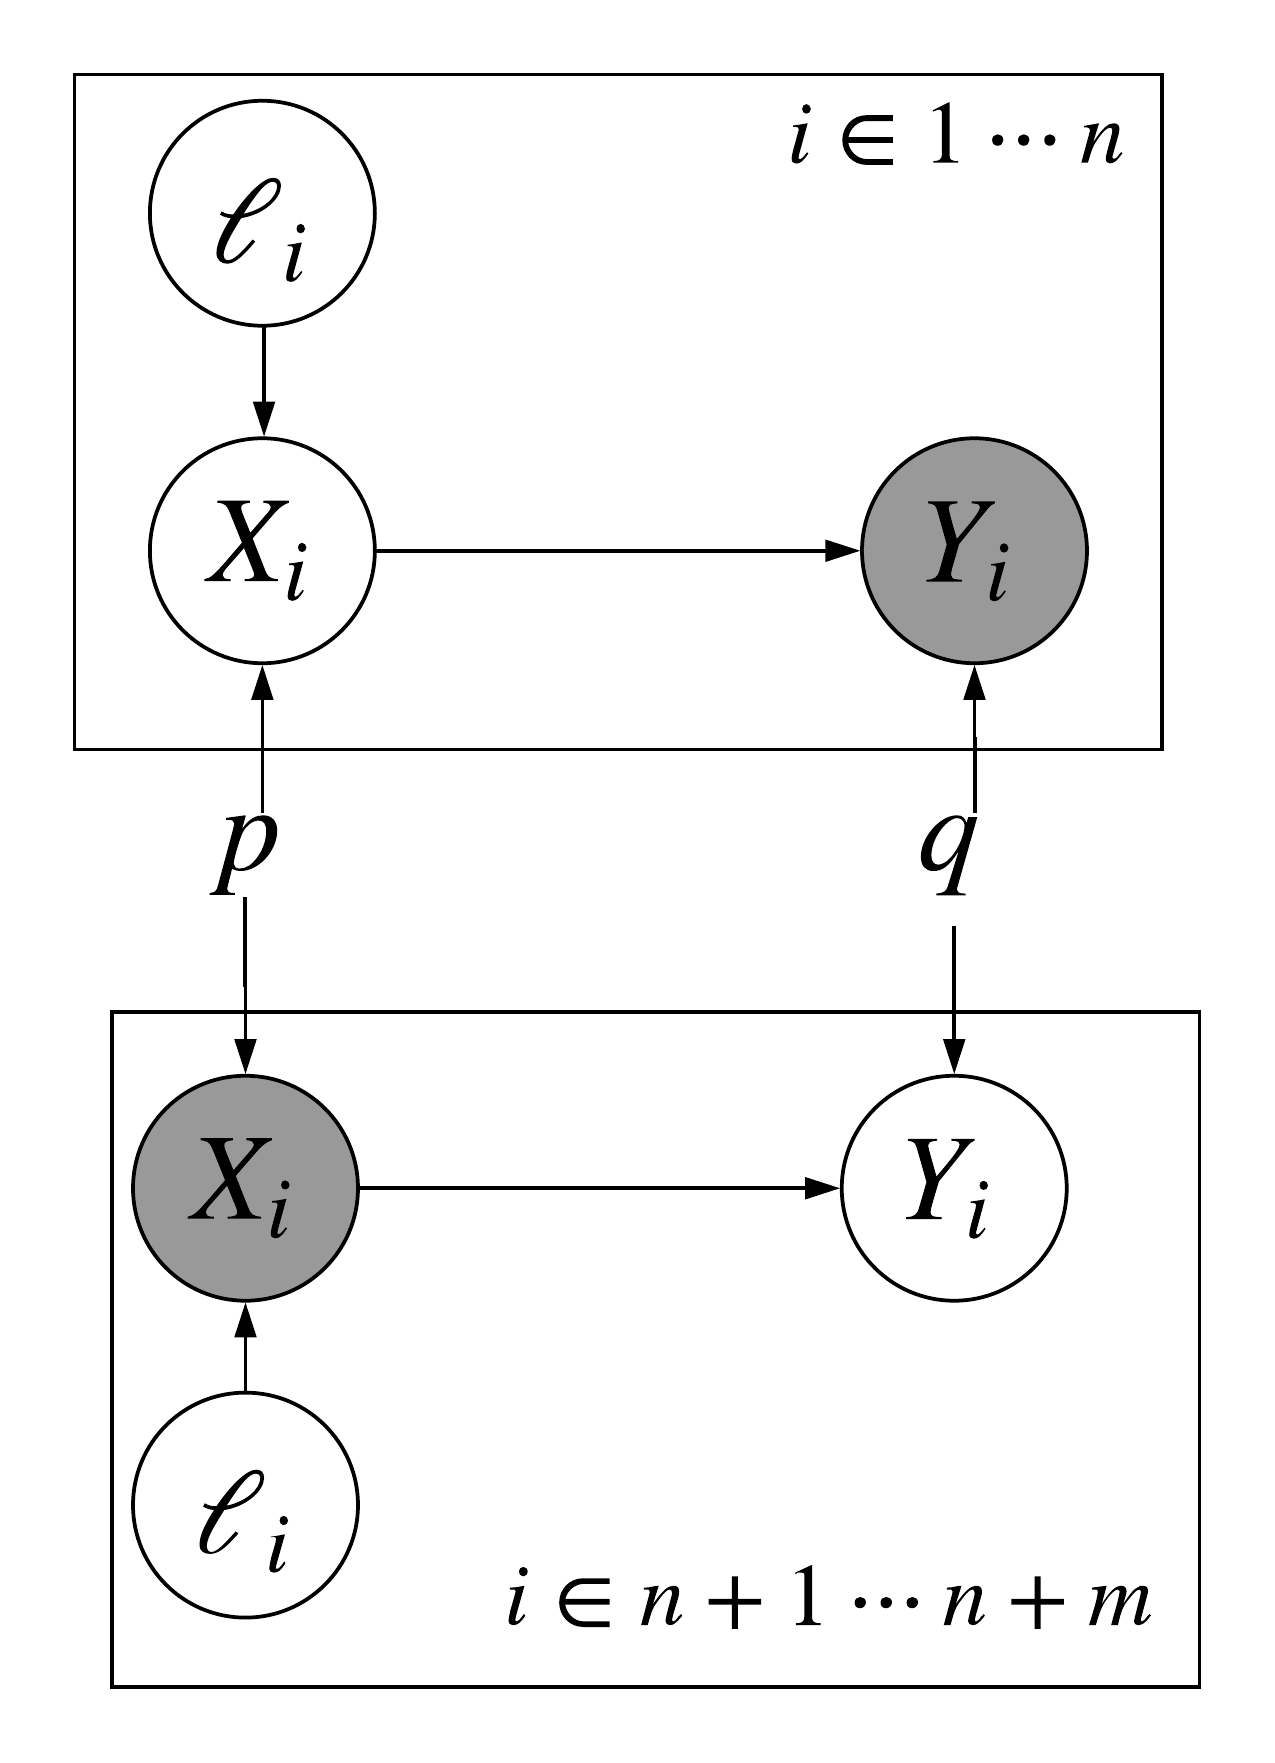
\includegraphics[width=.3\textwidth]{pics/plate}\hfill{}
\caption{We assume that we have two datasets, drawn from different techniques applied to specimens from various subpopulations.  In the top dataset, the results of technique II, denoted by $Y_i$, are hidden from us (we indicate this by making the circle gray).  In the bottom dataset, the results of technique I, denoted by $X_i$, are hidden from us.  In each dataset, we know what subpopulation of specimens we are considering, and this is designated by $\ell_i$.  Thus, for any given specimen $i$ we can observe either $\ell_i,X_i$ or $\ell_i,Y_i$ but never $\ell_i,X_i,Y_i$.  Using observations of $X_i$ we can certainly learn the parameters $p$ which govern the relationship between $X_i$ and the subpopulation, $\ell_i$.  Likewise we can determine the relationship between $Y_i$ and $\ell_i$.  However, if we believe that the relationship between $X$ and $Y$ is the same regardless of the population value $\ell$, we can also learn something about the parameters $q$ which govern the relationship \emph{between} $X$ and $Y$.\label{fig:plate}}
\end{figure}

Mathematically, we formulate our model as follows:

\begin{itemize}
\item Let us say we have $n+m$ individual members of a population.  These could be cells, humans, or whatever the smallest sample unit may be for a given problem.
\item For each individual member, we have some readily observable features by which we can group the members, such as the size of a cell, where an individual lives, or some other basic information.  We designate these features as $\ell_i$ for the $i$th individual.
\item For the first $n$ members, we have made an observation using the first technique.  This gives us the values $X_1 \cdots X_n$.
\item The last $m$ members were observed using the second technique.  This gives us the values $Y_{n+1} \cdots Y_{n+m}$.
\end{itemize}

For simplicity, we here assume that $\ell_i,X_i,Y_i$ take values in finite sets, $\Omega_\ell,\Omega_X,\Omega_Y$.  Extensions to more general cases should be straightforward, but we must leave them to future work.  

We further posit a set of \emph{counterfactual} variables -- variables which could not ever be obtained in practice, but which help us organize our thinking.  These are sometimes referred to as ``potential outcomes''  (cf. \cite{rubin2005causal}).

\begin{itemize}
\item Let $Y_1 \cdots Y_n$ denote the observations we \emph{would have gotten} if we had applied the second technique to the first $n$ members.
\item Let $X_{n+1} \cdots X_n$ denote the observations we would have gotten if we had applied the first technique to the last $m$ members. 
\end{itemize}

Our main assumption is a kind of Markov assumption, from which we obtain the name ``Markov Link Method'':

\begin{equation}\label{eq:mainassumption}
\mathbb{P}(X_i=x,Y_i=y|L_i=\ell)=p^*(x_i|\ell_i)q^*(y_i|x_i)
\end{equation}

for some distributions $p^*,q^*$.  Moreover, we assume that the vectors $\{(p^*(x_1|\ell)\cdots p^*(x_n|\ell))\}_\ell$ are linearly independent.  If this seems unlikely, it may make sense to collapse similar values of $\ell$ together.  The Markov assumption can be visualized with the plate diagram found in Figure \ref{fig:plate}.

The validity of these assumptions for a given situation should be closely contemplated.  There are several key questions to answer when deciding whether this assumption is applicable.  Does the process by which samples are gathered gathered depend only upon $\ell$?  In particular, is it not at all statistically related to which measurement technique was  applied, except through $\ell$?  Are the particular measurement biases of both techniques the same for every value of $\ell$?  Is the statistical relationship between the quantities being measured by the two techniques the same for every value of $\ell$?\footnote{Note that this is automatically true if both techniques are measuring the same thing.  More generally, if two techniques have something that they both measure, we can restrict attention to that one common phenomenon.}  If the answer to all of these questions is yes, the assumption that $(X_i,Y_i)$ is drawn from $p(x_i|\ell_i)p(y_i|x_i)$ may apply.  If some answer is no the method may still apply, but certain corrections may be necessary; we discuss these in our conclusions.

Under these key assumptions, the Markov Link Method gives us a way to uncover something about the relationship between the observations $X_i$ from one measurement technique and the observations $Y_i$ from the other measurement technique, i.e. the distribution $q^*$.  Unfortunately, given the limitations of the data, $q^*$ itself may be dramatically unidentifiable in many cases.  Instead, the Markov Link Method yields a \emph{set} of possible values of $q$ which are consistent with the data.  It can then be shown that the true value $q^*$ lies close to this set with high probability.  

To understand the limitations of the data more clearly, consider the case that $\ell$ lies in the set $\{1,2\}$, $X$ lies in the set $\{1,\cdots 100\}$ and $Y$ lies in the set $\{1,2\}$.  As long as $m,n$ are large enough, we can effectively estimate $p^*$ and $h^*(Y|\ell)=\sum_x p^*(x|\ell)q(Y|x)$.  However, this does not tell us very much about what $q$ might be.  Indeed, $q$ lies in a 100-dimensional space, and the restriction that $q$ must satisfy $h^*(Y|\ell)=\sum_x p^*(x|\ell)q(Y|x)$ for each $(\ell,Y)$ actually only introduces 2 new constraints.  Thus there is a 98-dimensional space that $q$ may lie in, and we simply cannot know where in that space $q$ may lie.  However, in practice, we find that the \emph{inequality constraints}, namely that $q(y|x)\geq0$ for every $(x,y)$, can actually force this potentially vast space to be tightly centered around a single point.  

In formal terms, the Markov Link Method produces a estimator for the set of possible values of $q$ which are consistent with what is observable, i.e.

\begin{equation*}
\Theta^* \triangleq \left\{q:\ \sum_y p^*(x|\ell)q(y|x) = \sum_y p^*(x|\ell)q^*(y|x)\ \forall \ell,y\right\}
\end{equation*}

Let us see now how MLM achieves this.

\section{Algorithm}

The Markov Link Method begins by estimating

\begin{itemize}
\item $p^*$ using the empirical distribution of the observations $\{X_i\}$, $\hat p(x|\ell)$
\item $h^*(y|\ell)\triangleq \sum_x p^*(x|\ell)q^*(y|\ell)$ using the empirical distribution of $\{Y_i\}$, $\hat h(y|\ell)$
\end{itemize}

These empirical distributions may not be quite consistent with the original assumption that the distribution of $X,Y|\ell$ may be written as $p^*(x|\ell)q^*(y|x)$.  In particular, it may be that there is \emph{no} value of $q$ such that $\sum_x \hat p(x|\ell) q(y|x) = \hat h(y|\ell)$.  There may also be many such values.  To obtain a well-defined estimator, we take a value of $q$ which is decent, and use a slight regularization to ensure it is uniquely defined.  Let $N_{X,\ell}=\#\{i\leq n:\ \ell_i=\ell\},N_{Y,\ell}=\#\{i> n:\ \ell_i=\ell\}$.  We take
%
\begin{equation*}
\hat q = \argmax_q \sum_\ell N_{Y,\ell}\sum_{y}\hat h(y|\ell)\log\left(\sum_{x}\hat p(x|\ell)q(y|x)\right) + \kappa \sum_{xy} \log q(y|x)
\end{equation*}
%
In practice, we took the entropic regularizer $\kappa$ to be $0.01$; it is mostly useful for ensuring numerical stability of the algorithm.  

This method gives us an estimate for $\hat q$, but we emphasize this estimate is very likely to be \emph{inconsistent} for the true value of $q^*$.  As we described in the previous section, this is simply a limitation of the data we have available -- attempting to deduce $q^*$ may be too much to ask for.  However, subject to suitable assumptions, the estimator
\begin{equation*}
\hat \Theta\triangleq \left\{q:\ \sum_y \hat p(x|\ell)q(y|x) = \sum_y \hat p(x|\ell)\hat q(y|x)\ \forall \ell,y\right\}
\end{equation*}
is indeed consistent in the sense that we can be asymptotically assured that the true $q^*$ lies very close to some point in $\hat \Theta$.

\vspace{.1in}
\begin{thm}
Fix any $\kappa>0$.  Let $N_{X,\ell},N_{Y,\ell}\rightarrow\infty$ in such a way that $N_{Y,\ell'}/\sum_{\ell}N_{Y,\ell} \geq \rho>0$ for each $\ell'$.  Let us assume that $q^*(y|x)>0$ for every $x,y$ and the rows of $p^*$ are linearly independent.  Then $\inf_{q\in \hat\Theta} \sup_{x,y}|q^*(y|x)-q(y|x)|\rightarrow 0$ in probability.
\end{thm}

\begin{proof}
We defer the proof to Appendix \ref{sec:proof}.
\end{proof}

We close by remarking that the assumption $q^*(y|x)>0$ is very likely to be unnecessary.  However, it substantially simplifies the proof.  We therefore leave a more complete theorem for future work.  

\section{Empirical results}

\begin{figure}
\begin{minipage}[c]{.3\textwidth}
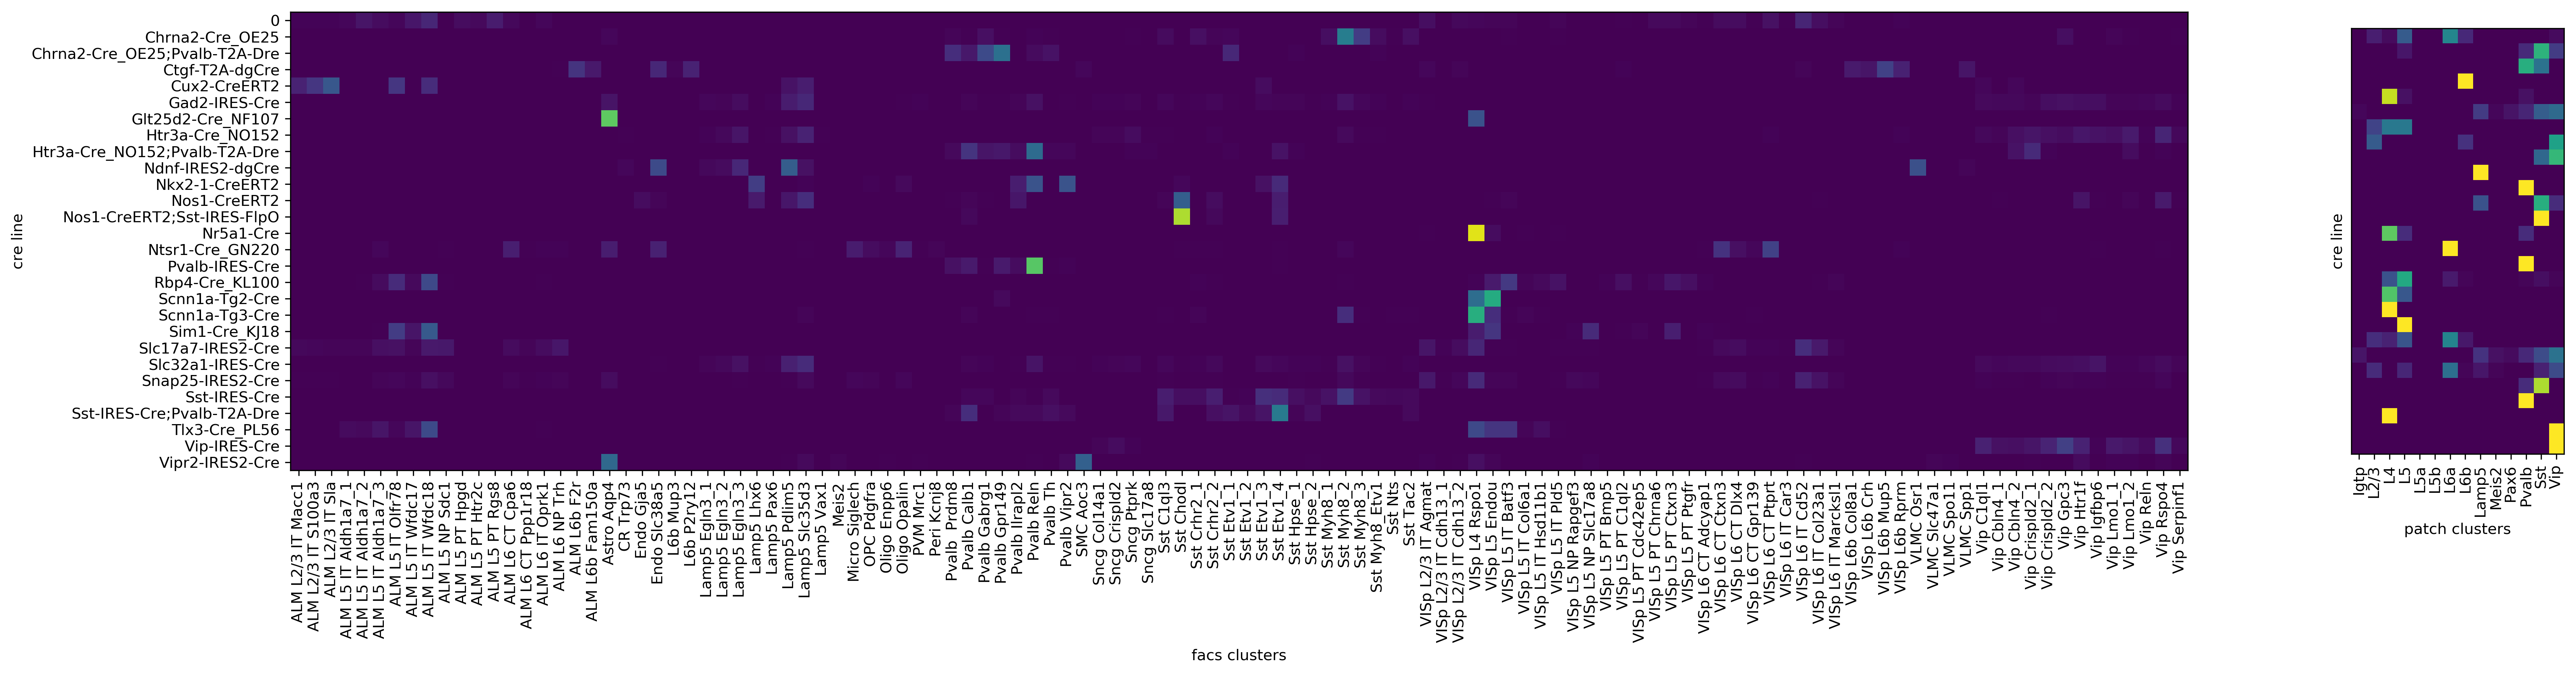
\includegraphics[width=.9\textheight,angle=270]{pics/alleninput}
\end{minipage}
\hfill
\begin{minipage}[l]{.4\textwidth}
\caption{Input: two tables.  The Allen Institute had access to various cre-line-based cell selection techniques.  Each technique pulls out a different group of cells.  Once the cells were selected, they were then either subjected to technique I (`facs') or technique II (`patch').  Technique I gives a very complete analysis of the gene expression of the cell.  Technique II gives a less complete analysis, but yields additional electrophysiological data that may be of interest.  The results of technique I was used to assign cells to one of 116 categories, and the results of technique II was used to assign cells to one of 14 categories.  The tables above show the distribution of category assignment for each sub-population selection technique.  The goal is to use these tables to be able to say something about how the 14 categories from Technique II might line up with the 116 categories from technique I.  \label{fig:alleninput}}
\end{minipage}
\end{figure}

Our motivation for this problem arose from looking at Allen Institute cell-type assignment of cells, performed using two different experimental techniques (also called experimental ``modalities'').  The only thing connecting the two modalities was that each modality had a variety of samples drawn from a variety of sub-populations, and the same sub-populations were used for both modalities.  Thus our input was two tables: (technique I cell-type $\times$ sub-population), and (technique II cell-type $\times$ sub-population) (Figure \ref{fig:alleninput}).  A key question immediately appears from these tables: does the way in which we have clustered cells into different types under technique I line up nicely with the way in which we have clustered cells under technique II?  The Markov Link Method gives us a way of addressing this question that is completely agnostic about the underlying genetic markers that were used to produce the clusters.  Our output was a set $\hat \Theta$ of possible ways that technique I cell-types could line up against the technique II cell-types.  That is, each element of $\hat \Theta$ was itself a table of the form (technique I cell-type $\times$ technique II cell-type).

\subsection{Making sense of Markov Link Method output}

The Markov Link Method yields a set (indeed, a convex polytope).  Each element of this set gives a particular way that technique I might be related to technique II.  It is not immediately easy to understand how to use or visualize the polytope $\hat \Theta$ of possible values for $q$.  Ultimately we want to know something about the correspondence between the techniques, i.e. $q^*$ -- how can we make good use of a \emph{set} of possible corresponences?  Here we suggest several main tools for analysis:

\begin{itemize}
    \item Rotationally Uniform eXtremal samples (RUX).  Every point in the polytope is a convex combination of its vertices, so by understanding the extremal vertices of the polytope we understand much about what values are possible.  Unfortunatelly, there are a truly vast number of vertices, and looking at all of them is quite impossible.  Instead, we propose a method for drawing samples which are illustrative of the overall character of the polytope: Rotationally Uniform eXtremal samples.  These samples are drawn simply by selecting a random direction in the polytope, and finding the point in the polytope which is furthest along that direction.  With probability 1 this point is unique, and provides a useful notion of the polytope's extent.  Obtaining such a sample simply requires solving a linear programming problem.  We show 10 such samples in Figure \ref{fig:allenRUX}.  

    Each sample shows a possible way that the two different techniques might correspond; together, these samples reveal both what the data says about the correspondence and what we still need to know.  In particular, some entries of correspondence are nearly the same for every sample, and others can vary more significantly.  This suggests what possible experiments might be important to do next.  Since each row always sums to one, any ambiguity must lie in trading off between different columns within a row.  To resolve this ambiguity, we could find a subpopulation which we believe might include, say, half of those ambiguous columns, and then perform additional experiments in both modalities, drawing from that subpopulation.

    \item Diameter estimation.  One problem with RUX samples is that there may be some very special direction in which the polytope has tremendous width.  That is, simply looking at ten or twenty RUX samples or even taking standard deviations over thousands of RUX samples, it may appear that the polytope is quite small.  Yet, in fact, it may be that there is a very special direction such that if we travel along that direction we find a value of $q$ which is radically different from the typical RUX samples.  To assess this, we attempt to show the overall diameter of the polytope is fairly limited, thus convincing ourselves that this is not a problem.  In this effort, we obtained Paired Rotationally Uniform eXtremal samples (PRUX): we first choose a direction uniformly at random and then found the two extremal vertices on the polytope in that direction and in the opposite direction.  We then computed the distance between those vertices, as well as the distance between those vertices projected to the direction.  Doing this procedure many times and making a scatterplot yields Figure \ref{fig:allenwidths}.  This figure suggests that the polytope may be only about 8 units in diameter (although we caution that general results on polytope diameter estimation are not encouraging, cf. \citep{brieden1998approximation}).  Considering that the magnitude of this diameter would be distributed over 1624 entries of the matrix, each of which lies in $[0,1]$, it would seem that the polytope may indeed be a fairly small set.  Although there is certainly no guarantee that there isn't some very large-magnitude direction hiding within this polytope, it is encouraging that we do not find any extreme outliers in this figure.  

    \item Random uniform samples.  The maximum entropy principle provides a quite different point of view: given that we can never distinguish where $q$ may lie inside the polytope $\hat \Theta$, we could treat all such values of $q$ as equally likely.  In this vein, we apply a Dikin ellipsoid sampler to obtain samples drawn approximately uniformly from $\hat \Theta$.  We also look at the standard deviation of each entry of $q$ across all these samples, which gives us another way to assess where the polytope has significant ambiguity.  The results may be seen in \ref{fig:allenoutput}.
\end{itemize}

\begin{figure}
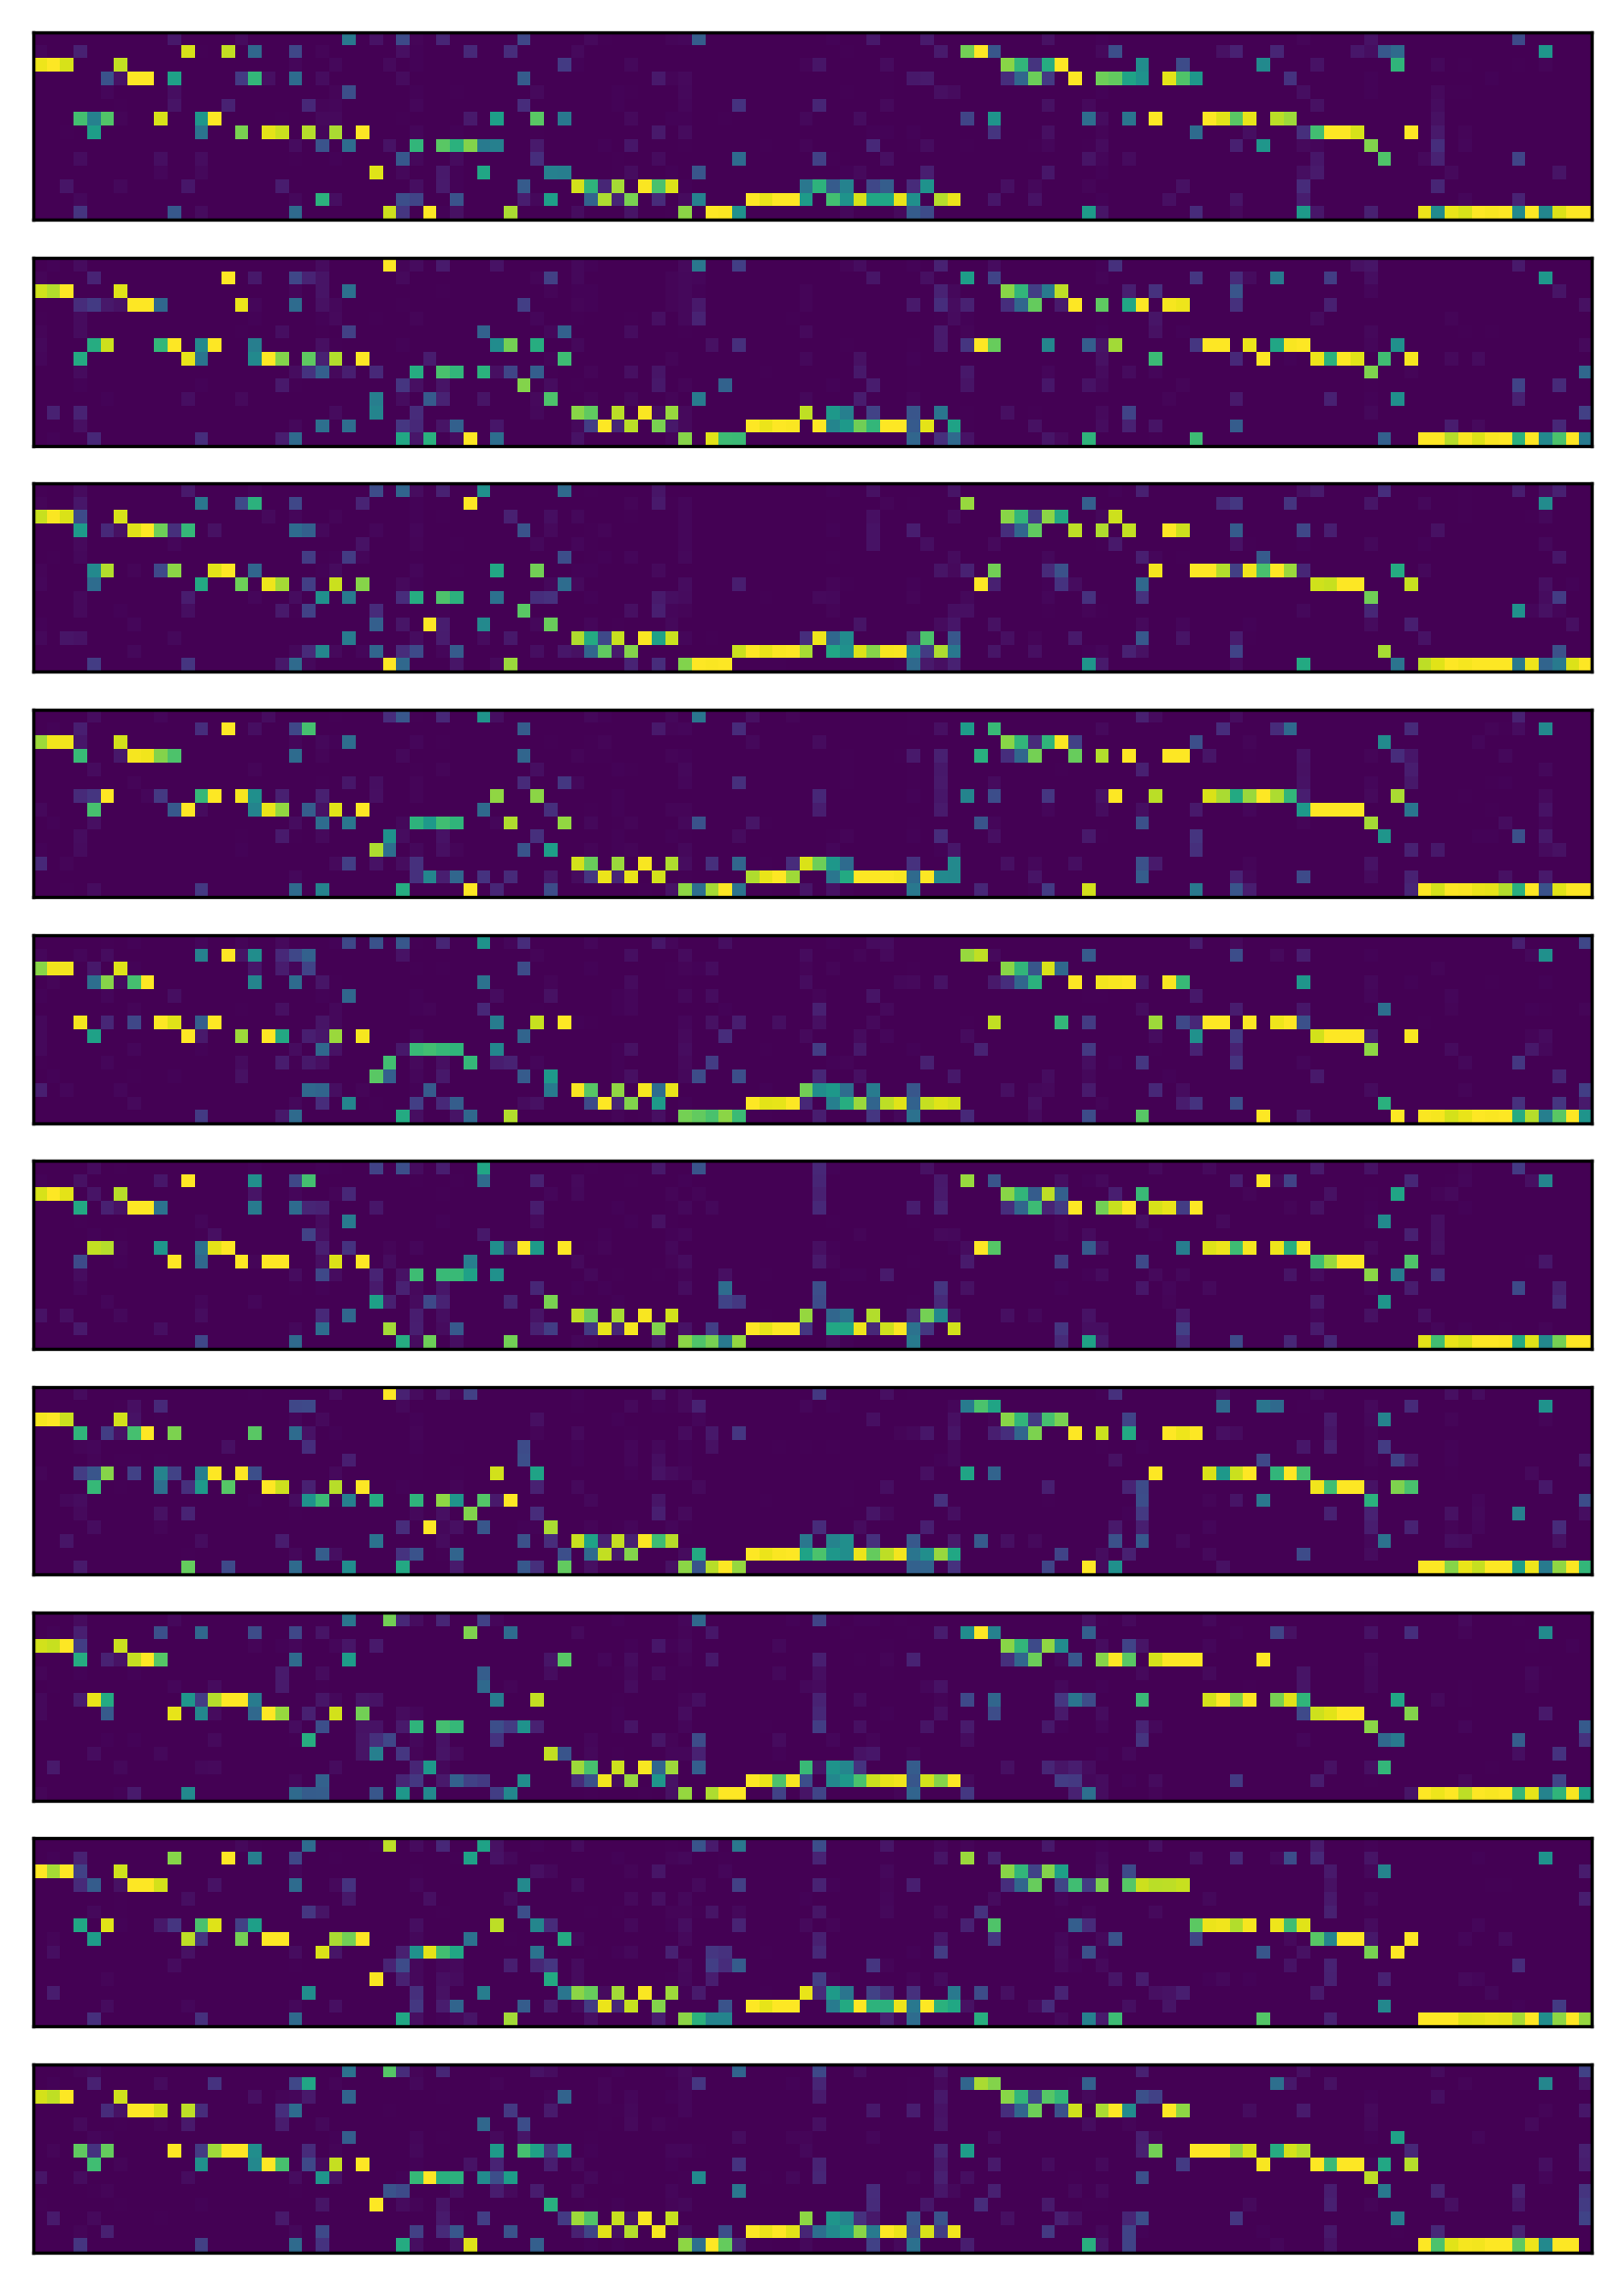
\includegraphics[width=0.8\textwidth]{pics/allenRUX}
\caption{10 Rotationally Uniform eXtremal samples from the polytope $\hat \Theta$.  These extremal samples from $\hat \Theta$ have quite a lot in common.  The common features are ones that we can feel confident are present in the true value of the joint distribution, $q^*$.  Other entries have more variability; these suggest specific experiments which might help disambiguate how technique I and technique II are related through $q^*$.  \label{fig:allenRUX}}
\end{figure}

\begin{figure}
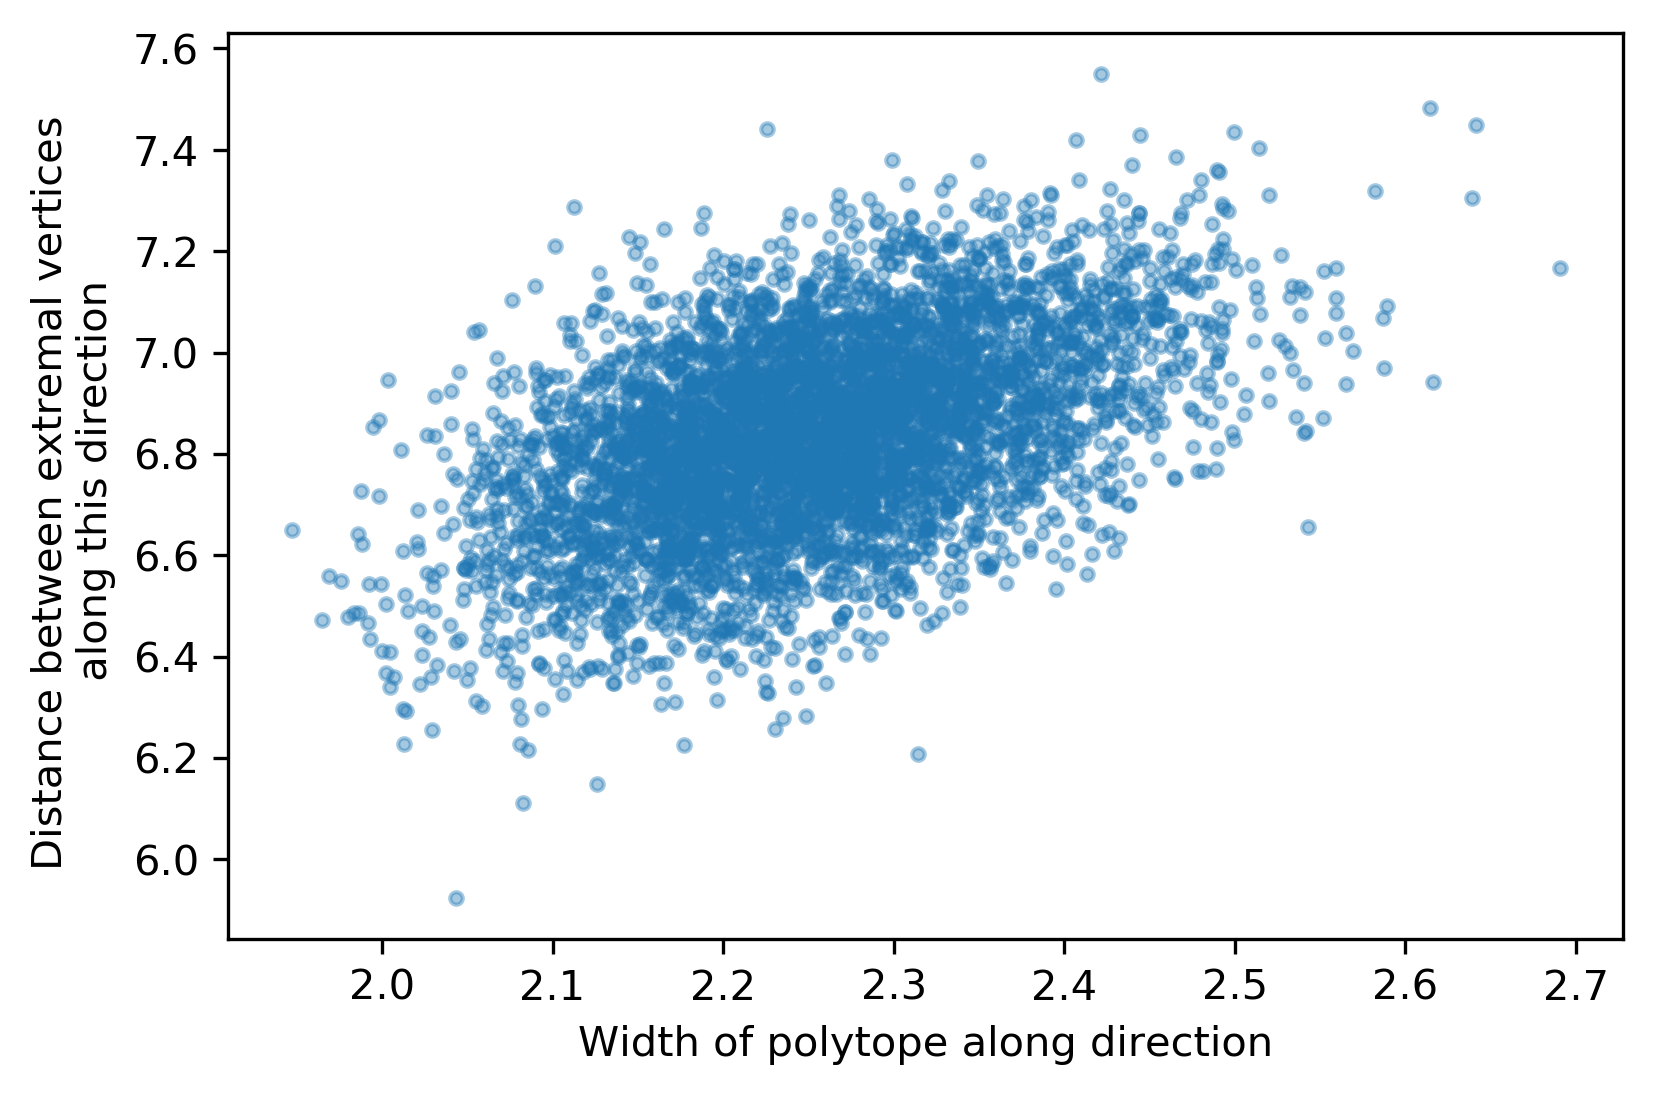
\includegraphics[width=0.8\textwidth]{pics/allenwidths}
\caption{How wide is $\hat \Theta$?  Each dot above corresponds to a randomly selected direction.  The horizontal position of the dot indicates the width of the polytope along that direction, and the vertical position indicates the distance between the two extremal vertices along that direction.  It appears that the overall diameter of the set may be less than 8 units.\label{fig:allenwidths}}
\end{figure}

\begin{figure}
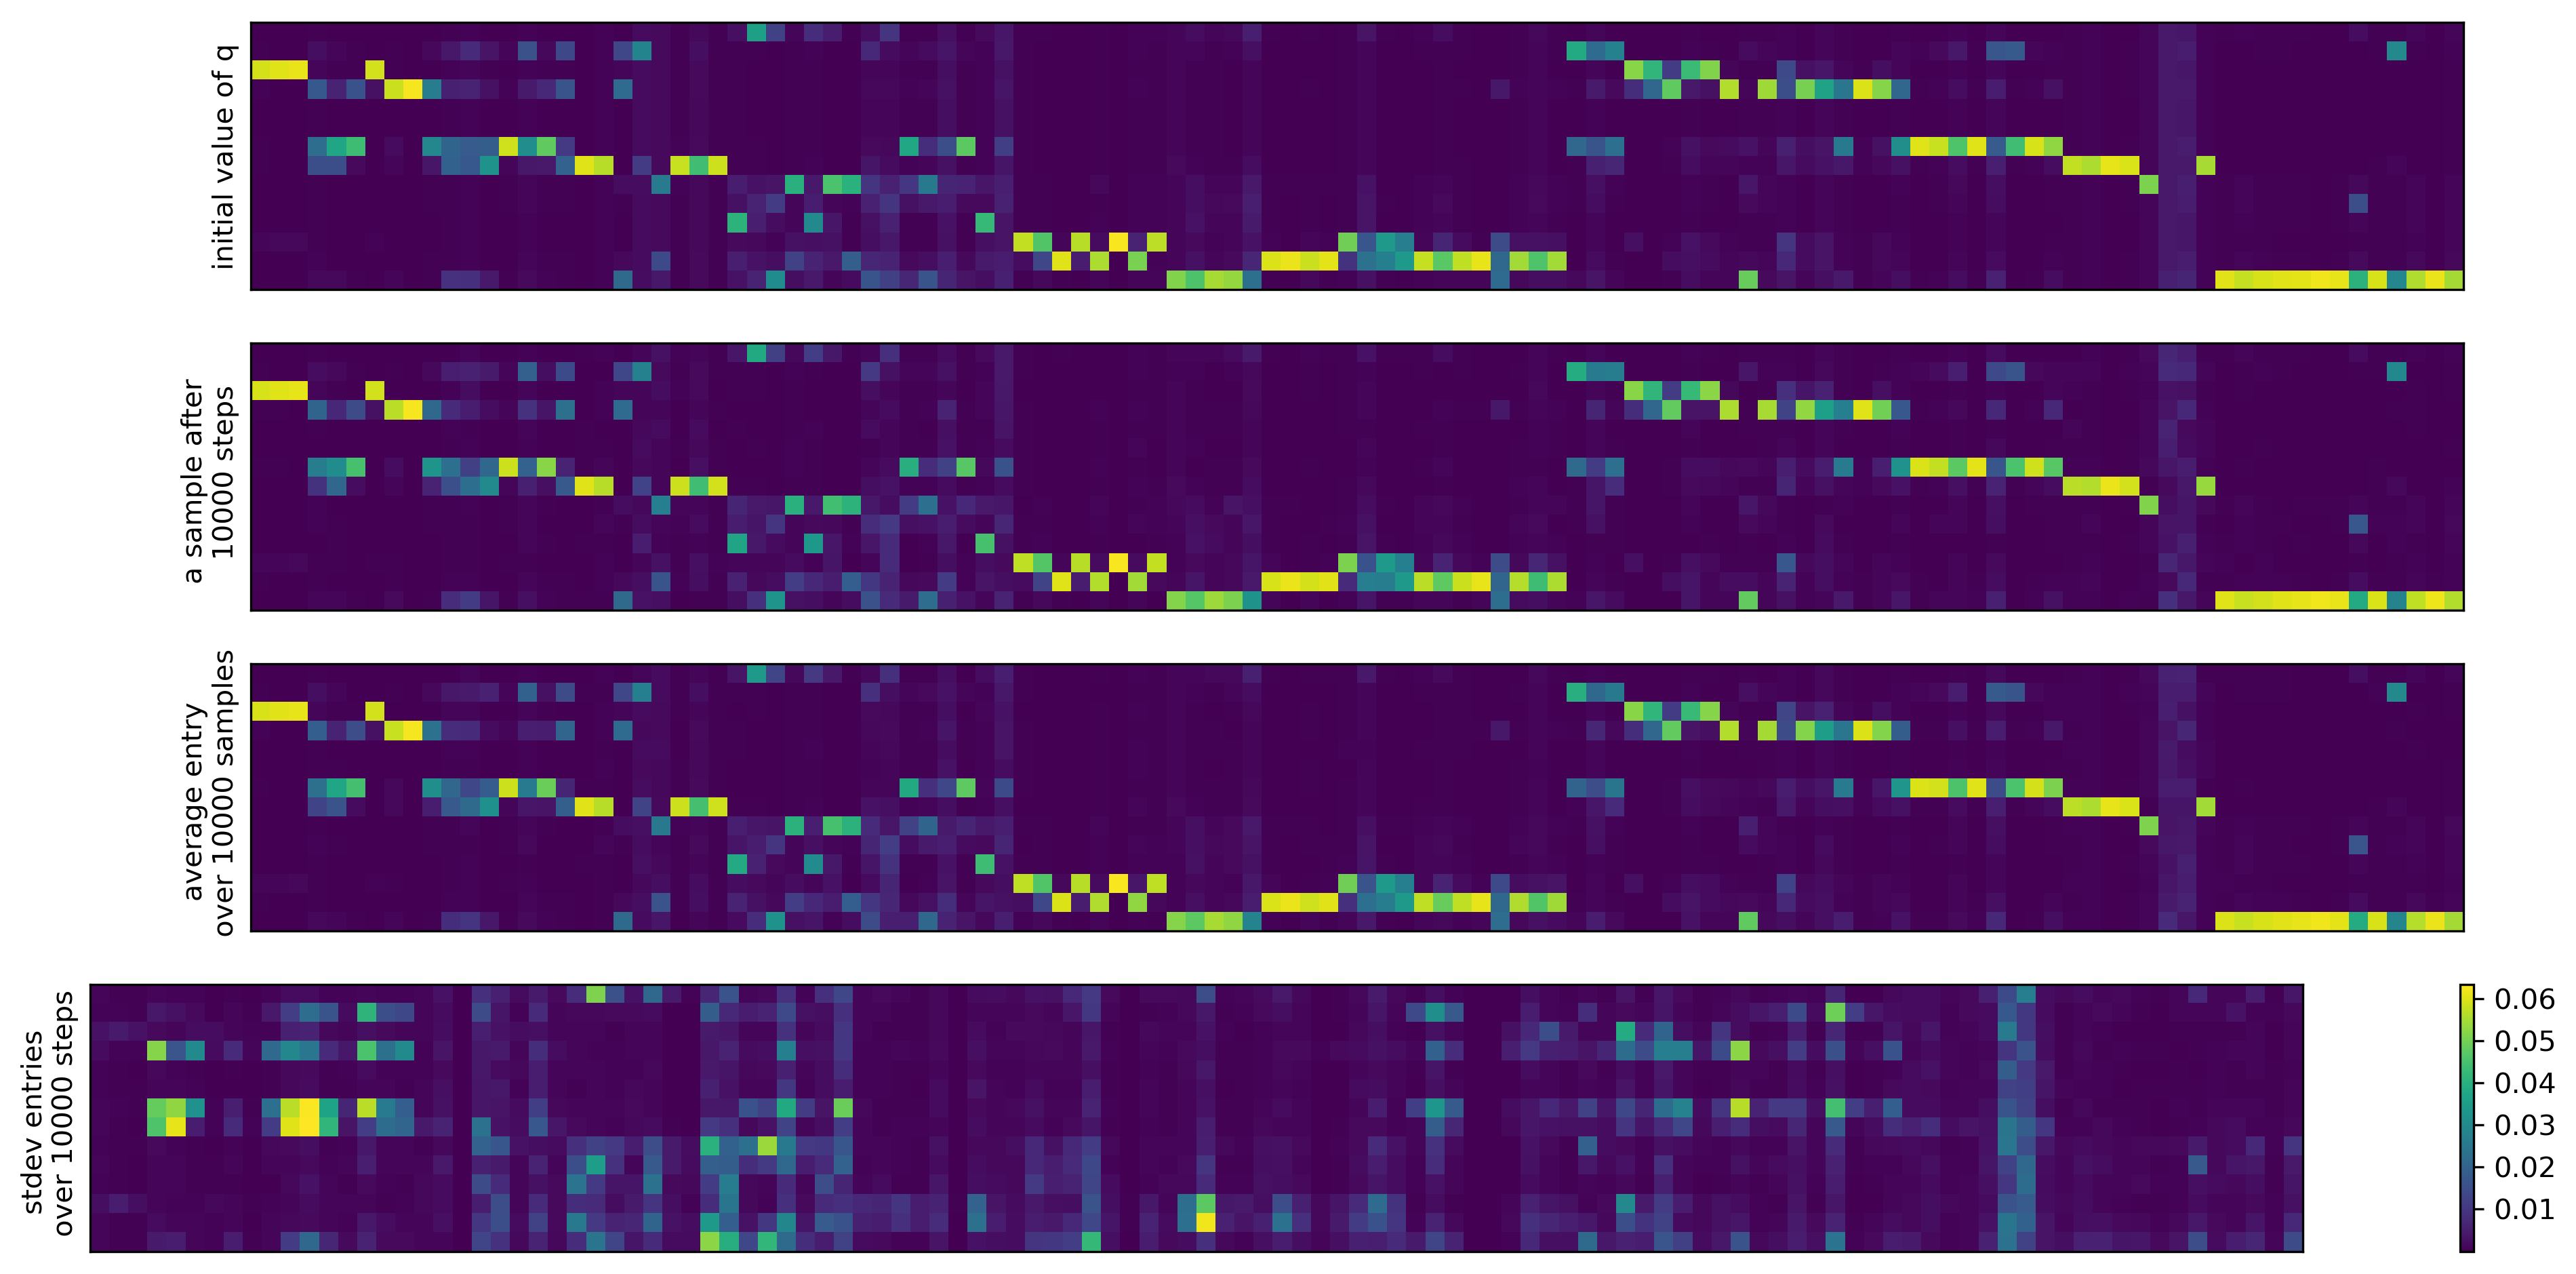
\includegraphics[width=0.8\textwidth]{pics/allenavg}
\caption{\label{fig:allenoutput}The first row shows the the MLM estimate of $\hat q$ (which is not a consistent estimator for $q^*$).  The second row shows a sample drawn approximately uniform from $\hat \Theta$, obtained by 10000 iterations of the Dikin sampler.  The third row shows the center of mass of $\hat \Theta$ and the final row shows the standard deviation of each entry (as estimated by the Dikin samples).  Notice that these deviations are never more than 6\%, suggesting that the polytope $\hat \Theta$ is closely centered around its center of mass.\label{fig:allenavg}}
\end{figure}

Together, these approaches give us practical ways of making real use of the results of the Markov Link Method.  More generally, they may be applied to many situations where a parameter of interest simply cannot be exactly identified but can be shown to lie near to some set.  

\subsection{Evaluation}

It is difficult to evaluate the accuracy of the Markov Link Method, because ground-truth data is not available in the cases where it actually matters.  Nonetheless, we can make a variety of attempts to see how the method fares.

Parametric bootstrap provides one natural way to assess our confidence.  That is, we simulate a surrogate dataset according to the estimated distribution (holding the number of samples for each group fixed), apply our method to the resulting surrogate dataset, and then obtain an estimate $\hat \Theta^{(i)}$.  We do this 100 times.  For each estimate, we can then measure whether the original $\hat q$ was is close to the estimated polytope, i.e. for each $i$ we can look at the Euclidean norm between $\hat q$ and the set $\hat \Theta^{(i)}$.  Doing so for 100 bootstrap samples and taking a histogram of these distances yield Figure \ref{fig:bootstrap}.  The results suggest our estimator has a fairly tight confidence around the true polytope $\Theta^*$ for this dataset.  However, we note that theoretical properties of this are certainly lacking.

\begin{figure}
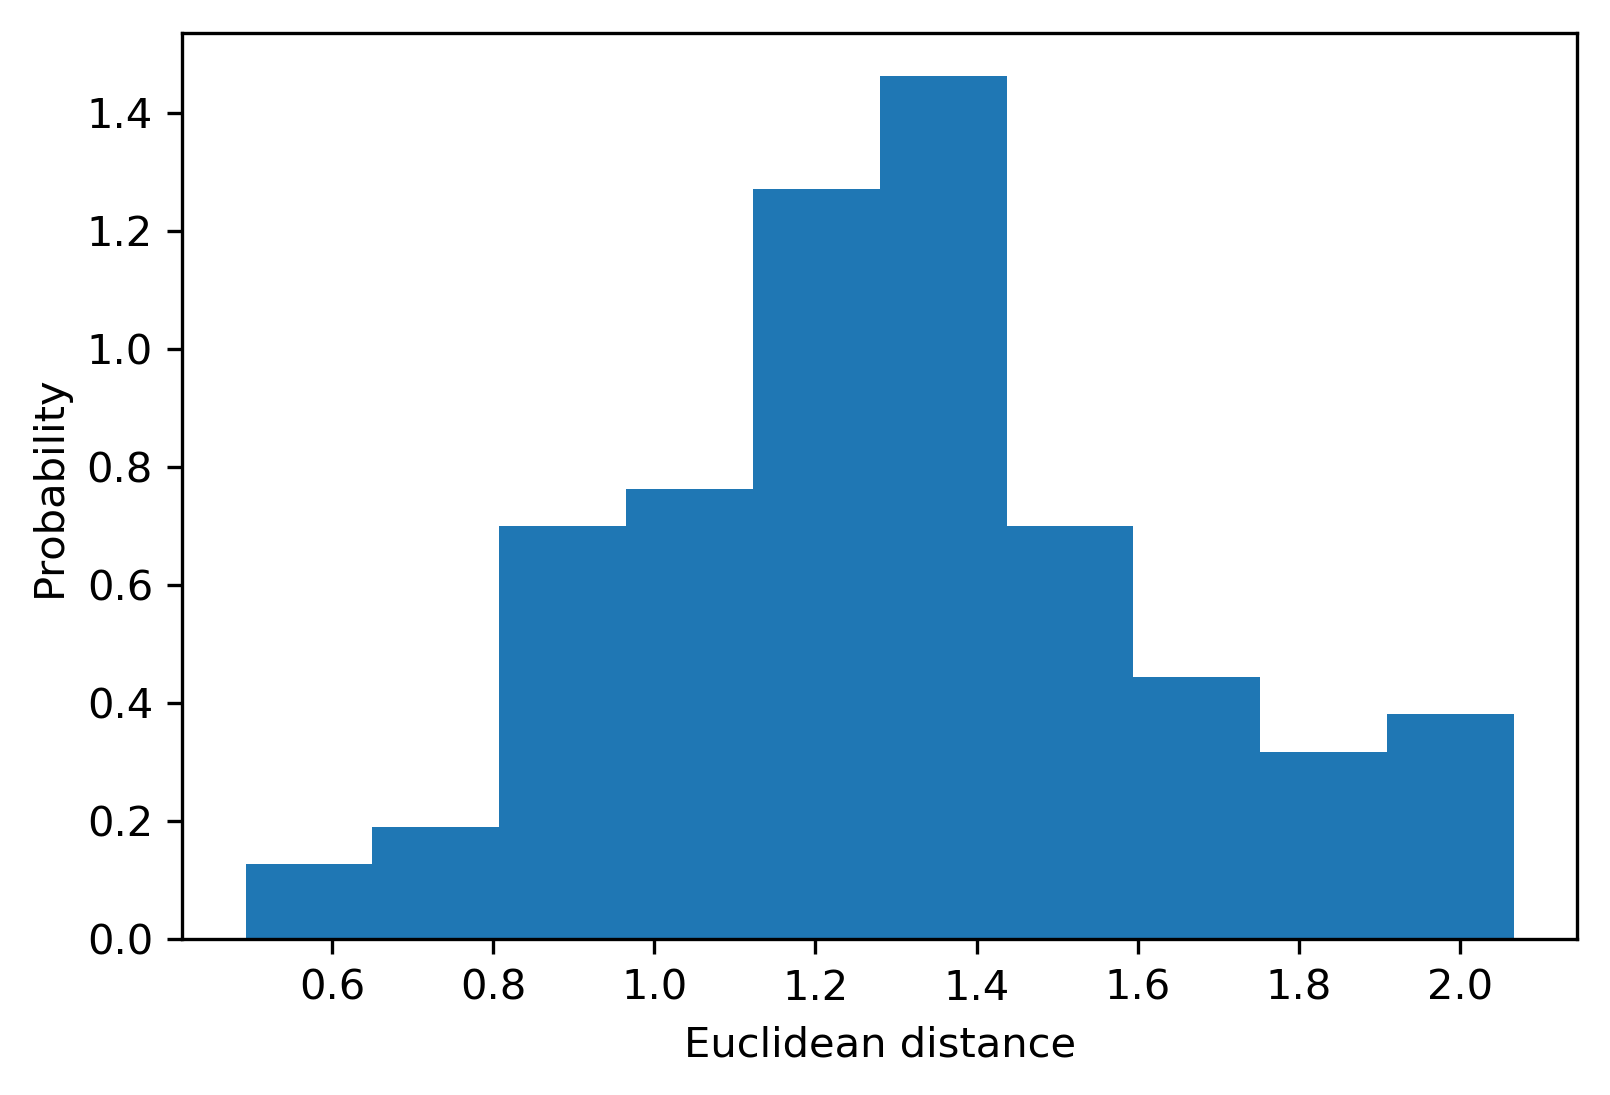
\includegraphics[width=0.8\textwidth]{pics/allenbootstrap}
\caption{Bootstrap gives us some measure of confidence in the MLM estimate.  None of the 100 bootstrap sample polytopes measured more than 2 units from from the original point estimate, $\hat q$.  That is, for each sample polytope we could find some point in the polytope that was less than 2 units from $\hat q$.  Spread out over the 1624 entries of the matrix $q$, each of which lies in $[0,1]$, we are encouraged insofar as 2 units does not seem to be a very great distance.  \label{fig:bootstrap}}
\end{figure}

Nonparametric bootstrap is another approach.  In this case, we simply sample the empirical distributions $\hat p,\hat h$ with replacement to obtain our surrogate datasets, and then apply the MLM method to each surrogate dataset.  We evaluate the degree of variability amongst the MLM polytope estimates by looking at the extremal points of those polytopes.  That is, we select a random direction and find the extremal vertex for each MLM estimate in that direction.  We can then look at position of these extremal points projected along that direction.  Looking over all the surrogates and subtracting the mean, we obtain a histogram of deviations.  We can then apply this to various directions, which yields the variety of histograms seen in Figure \ref{fig:allenbootstrap}.   

\begin{figure}
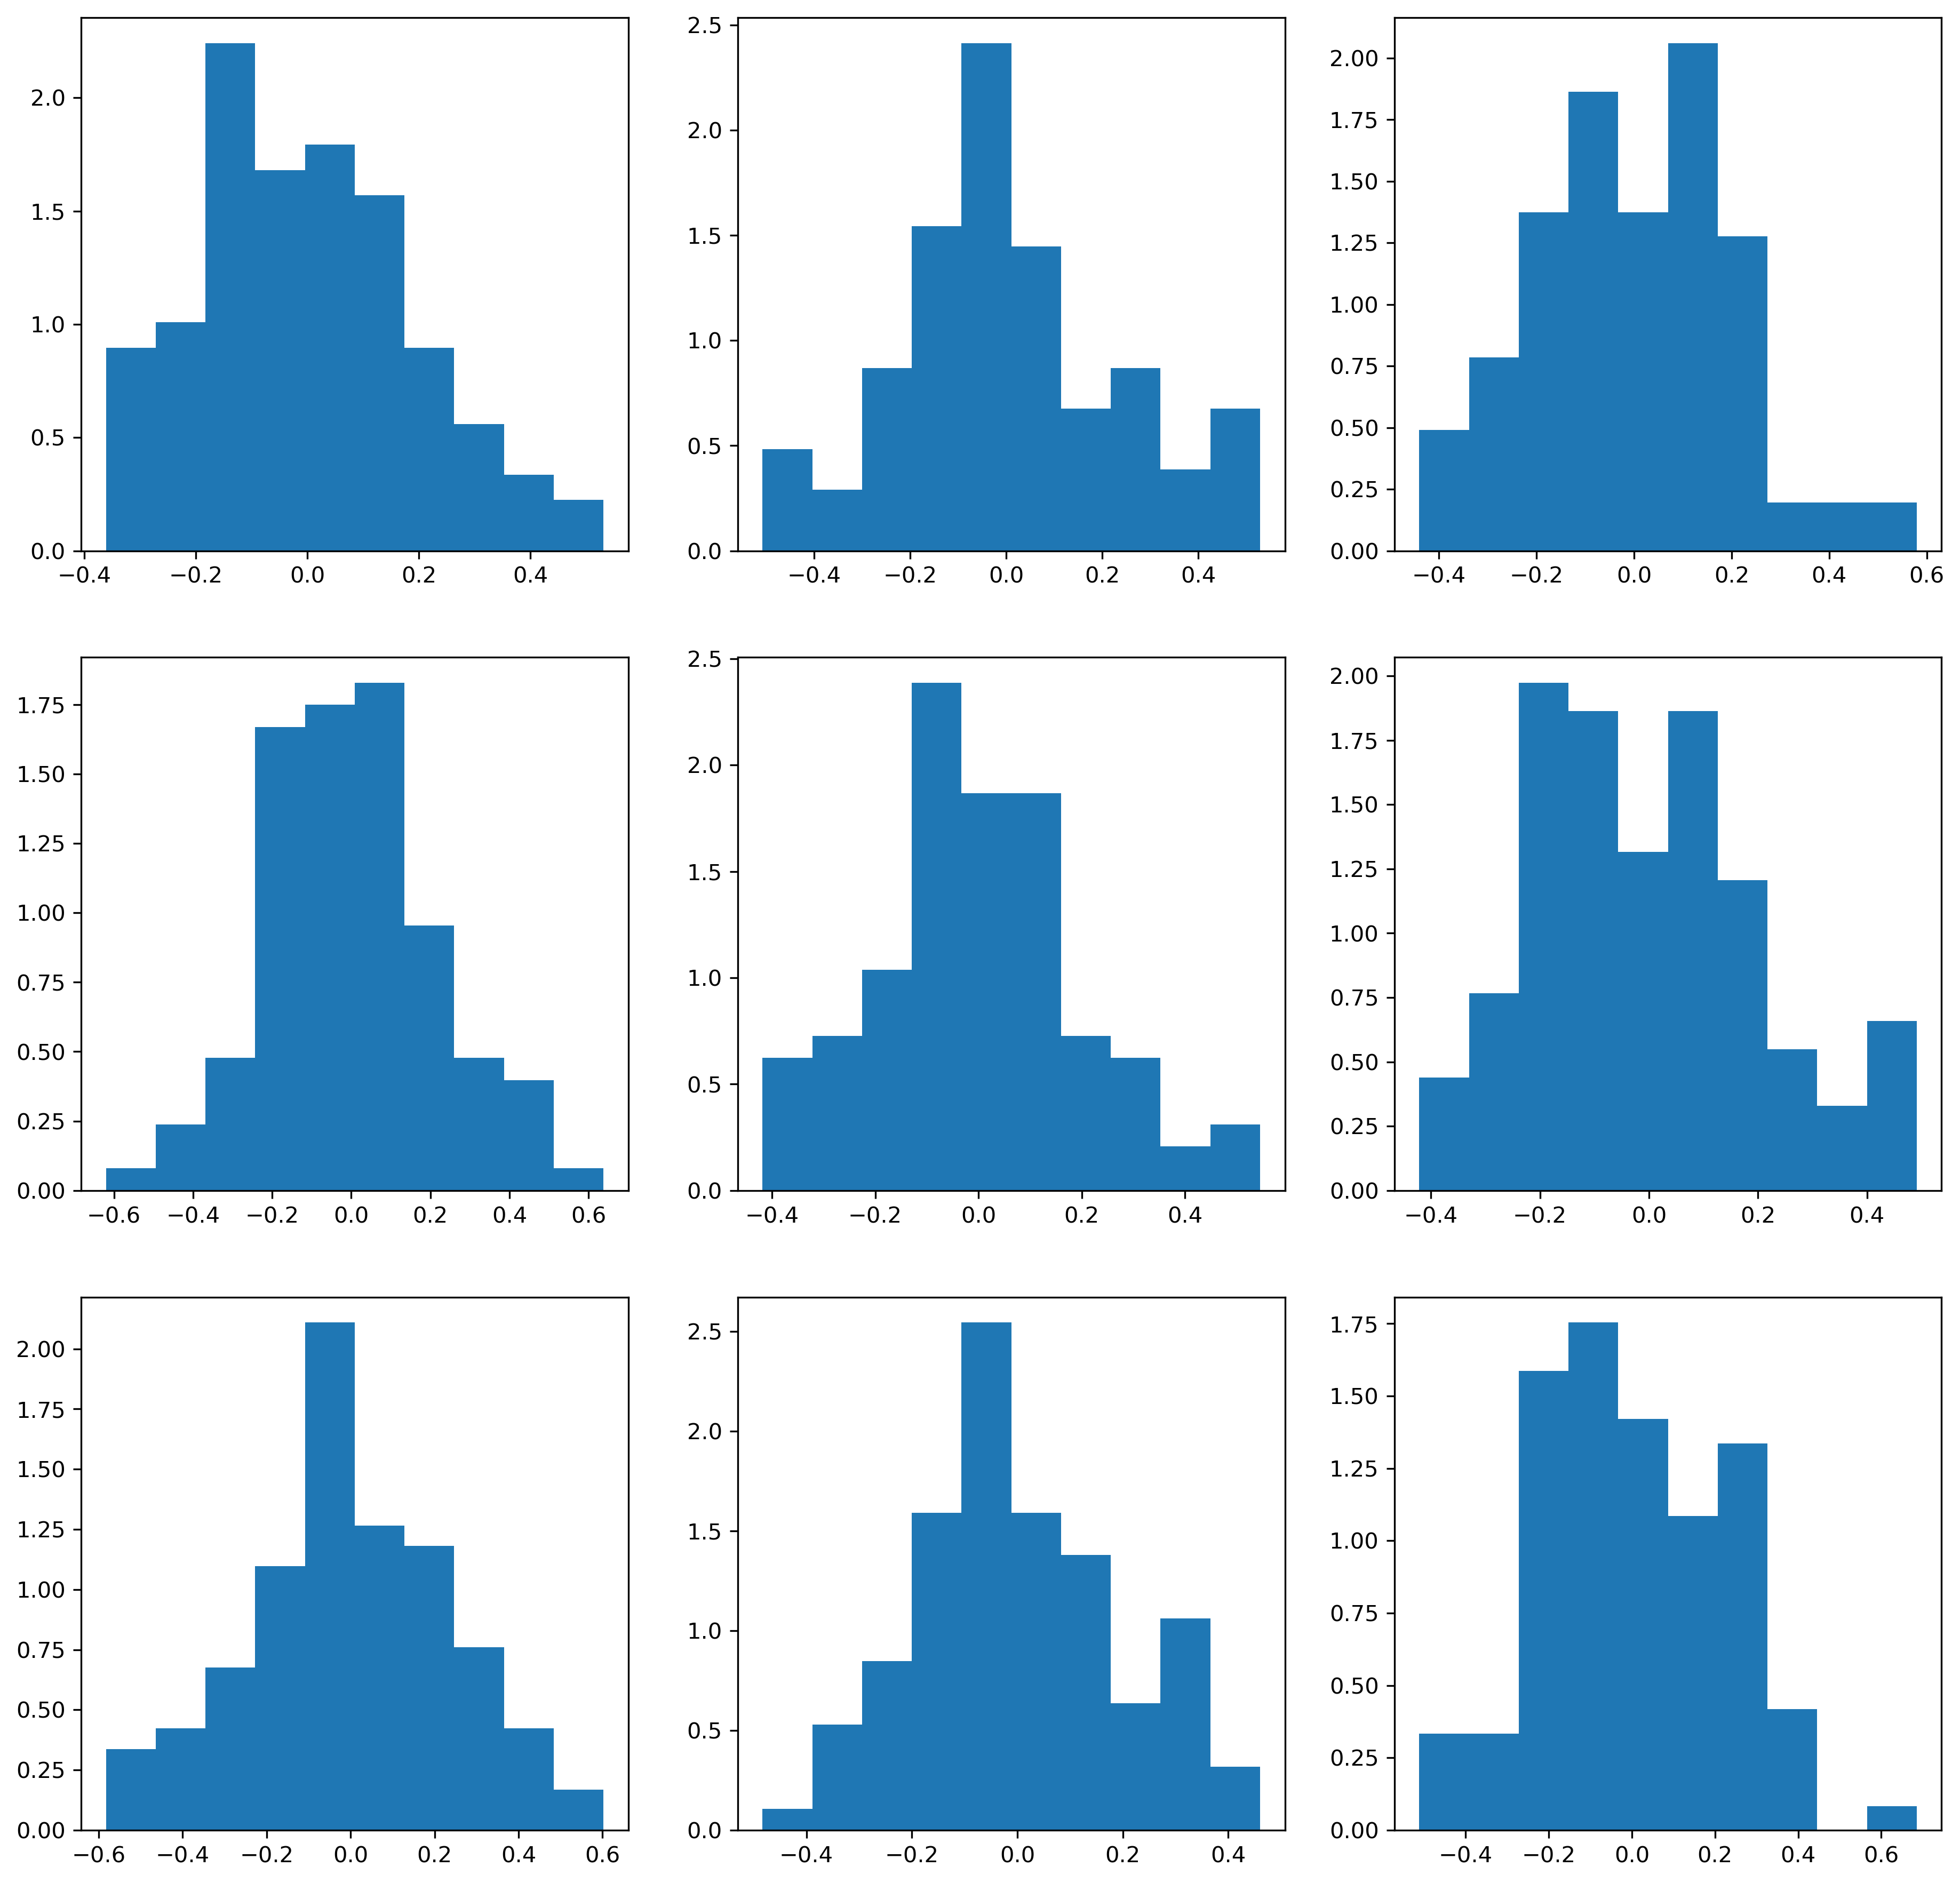
\includegraphics[width=0.8\textwidth]{pics/allenbootstrapnonparametric}
\caption{Nonparametric bootstrap gives us another form of confidence.  For each of nine randomly selected directions and for each bootstrap sample polytope, we compute how far the polytope extends in that direction.   For each direction we can then plot a histogram of how far the various polytopes extend.  We see that they do not vary dramatically between samples, which gives us confidence that our estimate is somewhat close to the truth.\label{fig:allenbootstrap}}
\end{figure}

Finally, we can look directly at whether MLM helps us model the data $Y$.  In theory it seems possible that by pooling data between the modalities we could gain statistical power.  This is particularly true in the case of the particular dataset we investigated, wherein obtaining samples for technique II is quite expensive and so there are far fewer available datapoints for the $Y$ data.  Thus the empirical distribution of $Y|\ell$ (namely $\hat h$) may in fact be a very poor estimator.  This suggests that perhaps we might consider the estimator $\tilde h(y|\ell)\triangleq \sum_x \hat p(x|\ell) \hat q(y|x)$ instead,  since it allows us to leverage knowledge gained from the plentiful samples of technique I.  To test this estimator, we held out 10\% of the $Y$ data.  We then applied the MLM method to obtain estimates $\hat p,\hat q$ and use those to produce $\tilde h$ as an estimator for the distributions of $Y|\ell$.  We then compare $\tilde h$ and $\hat h$ by calculating the log-likelihood of each estimator on the held-out data.  We found an average value of -1.1 per entry for the MLM estimator $\tilde h$, but the empirical distribution $\hat h$ yields a held-out log likelihood of $-\infty$ because there are examples in the testing set that are simply never seen in the training set.  Even if we use pseudocounts to smooth the empirical distribution, we never obtain likelihoods as good as we get using the model which shared data between the two experimental modalities (See Figure \ref{fig:heldout}).  Thus we see that sharing data between the modalities helps can help us estimate each modality more accurately, as well as enabling us to understand more about the connection between the modalities.

\begin{figure}
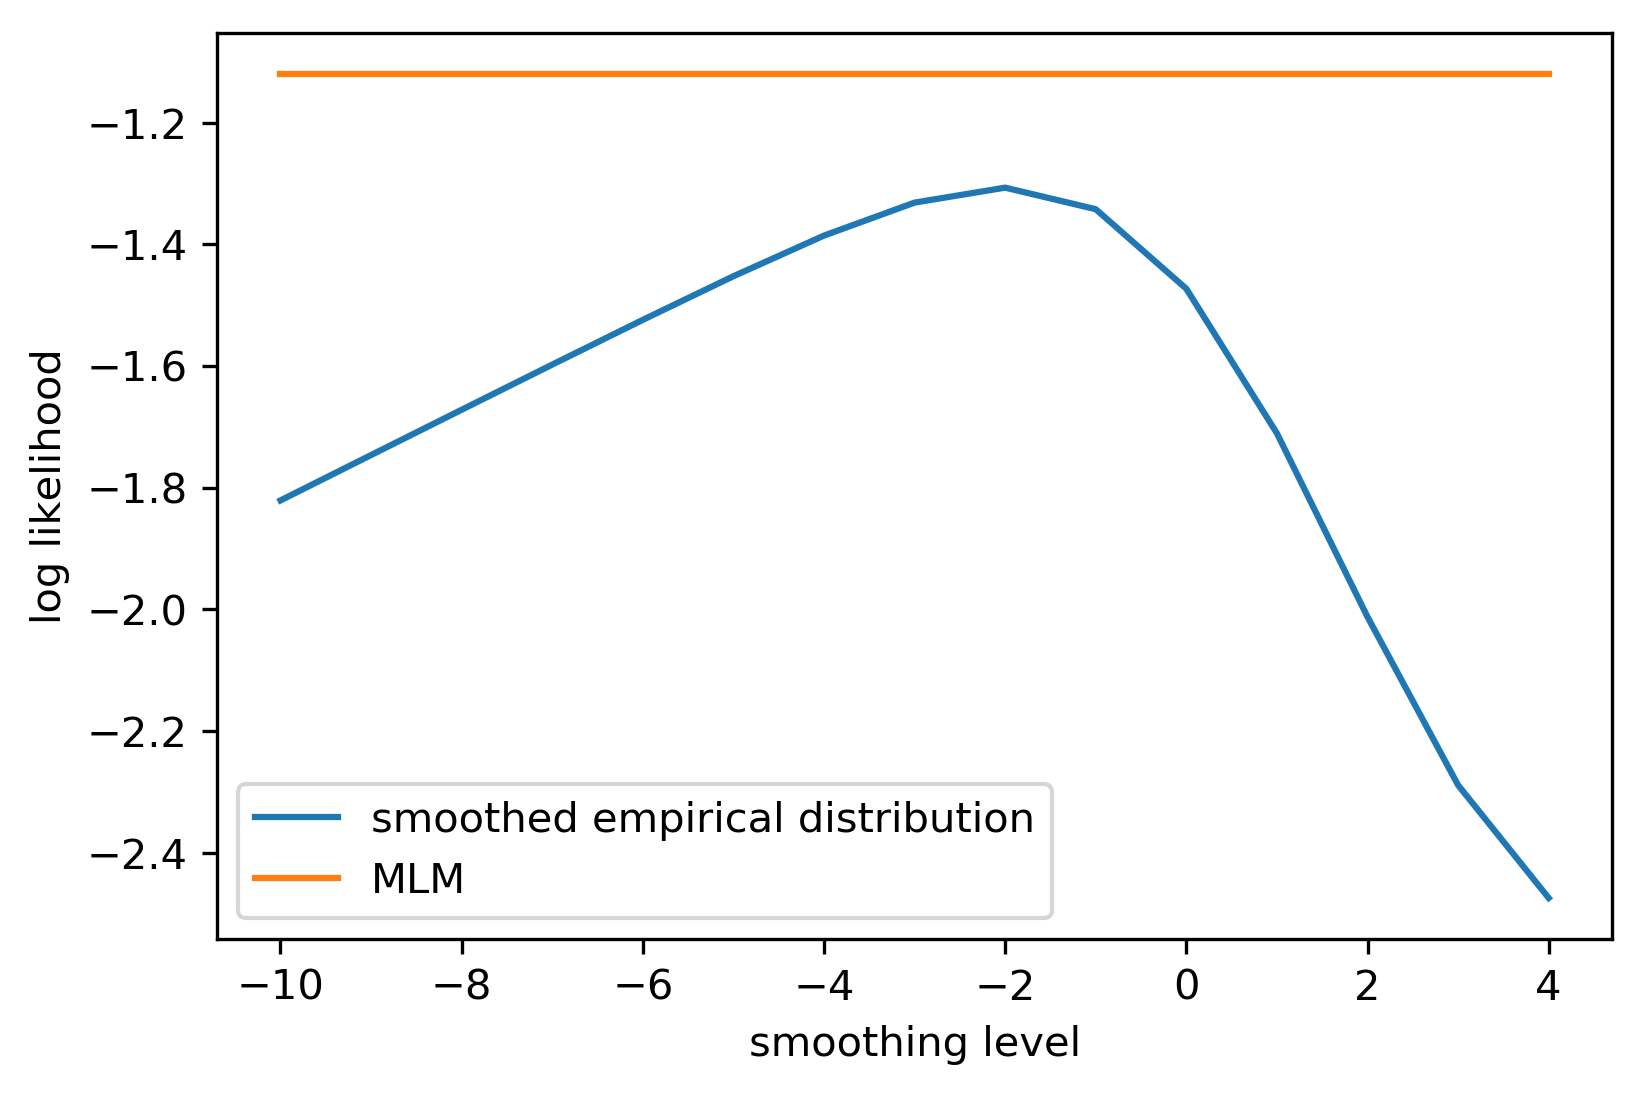
\includegraphics[width=0.8\textwidth]{pics/allenheldout}
\caption{Here we compare two estimators of the distributions of $Y|\ell$.  In the orange case, we use the Markov Link Method.  In the blue case, we use the empirical distributions of $Y|\ell$, smoothed using pseudocounts.  The horizontal axis indicates the size of these pseudocounts in log-scale.  The MLM method performs better than the empirical distribution at any level of smoothing. \label{fig:heldout}}
\end{figure}

\section{Conclusions}

When joint measurement is impossible, it can be difficult to calibrate two methods against each other or understand how they may be related.  Here we show that a simple Markov assumption can make it possible to actually learn quite a lot.  Although the exact relationship may not be identifiable, a polytope of possible relationships can be identified, and this polytope may in fact be quite small indeed.  By exploring this polytope, we can understand what we know -- and what we don't know -- about the relationship between measurements.

The Markov assumption is of course not the only one that we could have used, and may not be valid in every case.  For example, it has been speculated that some cell types tend to die more often in one experimental modality than another, and these cells are not part of the data.  This violates our assumptions.  However, assuming this death rate can be roughly measured, it can be adjusted for, yielding a different but equally meaningful assumption about the data.  Moreover, if this method yields bizarre results, it may give useful clues as to exactly how cell death may happen differently in the two modalities.

Once we accept that what we're interested in may not be fully identifiable, any of a wide variety of assumptions can help us obtain practical bounds.  Although we may not be able to learn exactly what we want, we can learn a set of possibilities.  By probing this set carefully with uniform samplers and extremal tests, we can learn what the data actually has to say and what experiments we need to do to learn more.  

\bibliographystyle{unsrt}
\bibliography{refs}

\appendix

\section{Dikin sampler}

\label{sec:dikin}

Consider a convex polytope $T=\{x:\ Ax\leq b\}$.  We have implemented a method for sampling from this polytope, based on the paper \citep{kannan2012random}.  This method makes use of the Dikin ellipsoids, $E(x)$.  For any $x$, these are defined by 

\begin{itemize}
    \item Computing the distance from $x$ to each facet of the polytope, i.e. $d_i = b_i - \sum_j A_{ij} X_j$.
    \item Constructing $\tilde A$ as $\tilde A_{ij} = A_{ij} / d_i$.
    \item Define $E(x) = \{y:\ |\tilde A (X-y)|\leq 1\}$.  
\end{itemize}

We can use these ellpsoids to efficiently sample the polytope $T$.    At each step, we have some point $X\in T$, and we would to use this point to obtain a new sample $Y$, such that by iterating this process we asymptotically obtain samples which are uniform in $T$.  Here is how we use $X$ to get $Y$:

\begin{algorithm}[H]
 \KwData{A point $X\in T$}
 \KwResult{A point $Y\in T$}
 \vspace{.1in}
  Sample a proposal $\tilde Y$, uniformly from $E(X)$\;
    \eIf{$X \in E(\tilde Y)$}{
        Sample $U \sim \mathrm{Uniform}[0,1]$\;
        \eIf{$U \leq \mathrm{Vol}(E(X))/\mathrm{Vol}(E(\tilde Y)) \leq 1$}{
            Let $Y \gets \tilde Y$\;
        }{
            Let $Y \gets X$\;
        }
    }{
        Let $Y\gets X$\;
    }
 \caption{Dikin sampler step}
\end{algorithm}

It is easy to show that the stationary distribution of the Markov chain found by iterating these Dikin sampler steps is indeed uniform on $T$.  To ensure an numerically robust method in the face of high-dimensional and nearly degenerate matrices, we take the following approach to robustly sampling from the ellipsoid:

\begin{algorithm}[H]
 \KwData{An $n\times m$ matrix $\tilde A$}
 \KwResult{A point $X$ sampled uniformly from $\{x:\ |Ax|\leq 1\}$}
 \vspace{.1in}
  Sample $Z$ as an $n$-dimensional normal variables vector\;
  Let $X$ denote the solution to the least squares problem $\min_x|\tilde Ax - Z|$\;
  Normalize $X$ by $X \gets X/|\tilde AX|$\;
  Sample $U \sim \mathrm{Uniform}[0,1]$\;
  Scale $X$ by $X \gets X \times U^{1/m}$\;
 \caption{Ellipsoid sampler}
\end{algorithm}


\section{Proof of the theorem}

\label{sec:proof}

For the benefit of the reader, we here repeat the statement of our theorem in more explicit terms.  

\begin{itemize}
\item Let $\UN{\cdot}$ denote the uniform norm (i.e.\ the maximum absolute value) and $\EN{\cdot}$ denote the Euclidean norm (i.e.\ the square root of the sum of the squares).  In the case of matrices, this Euclidean norm goes by the name of the Frobenius norm.  Recall that in this norm matrices satisfy a Cauchy-Schwarz like equality, $\EN{pq}\leq\EN{p}\EN{q}$.  Also recall that $\UN{a} \leq EN{a} \leq \sqrt{n}\UN{a}$ where $n$ is the number of entries in $a$.
\item Let $T_{a,b}$ denote the transition matrix polytope, i.e. the set of $a\times b$ matrices whose rows sum to 1 and whose entries are all positive.
\item Let $|\Omega_\ell|,|\Omega_X|,|\Omega_Y| \in \mathbb{N}$.
\item Let $p^*\in T_{|\Omega_\ell|,|\Omega_X|}$.
\item Let $q^*\in T_{|\Omega_X|,|\Omega_Y|}$.
\item We require the matrix $q^*$ has strictly positive entries, $q^*_{xy}\geq c>0$.
\item We require that the rows of $p^*$ are linearly independent.
\item Let $\hat p$ denote an empirical transition matrix drawn by obtaining $N_{X,\ell}$ samples for each row of $p^*$, i.e. we have samples $(\ell_1,X_1) \cdots (\ell_1,X_n)$ such that $\mathbb{P}(X_i=x) = p^*_{\ell_i,x}$, $N_{X,\ell}=\sum_{i=1}^n \mathbb{I}_{\ell_i=\ell}$, and $\hat p_{\ell x} = \sum_{i=1}^n \mathbb{I}_{X_i=x,\ell_i=\ell} / N_{X,\ell}$. 
\item Let $\hat h$ denote an empirical transition matrix drawn by obtainin $N_{Y,\ell}$ samples for each row of $h^*$.  
\end{itemize}

Now fix any $\kappa>0$.  Let
\begin{align}
\hat q = \argmax_q \left(\sum_\ell N_{Y,\ell}\sum_{y}\hat h(y|\ell)\log\left(\sum_{x}\hat p(x|\ell)q(y|x)\right) + \kappa \sum_{xy} \log q(y|x)\right)\label{eq:mindef}
\end{align}
and $\hat \Theta=\{q:\ \hat p\hat q=\hat pq\} \cap T_{|\Omega_X|,|\Omega_Y|}$.  
\vspace{.1in}
\begin{thm}
If $N_{X,\ell},N_{Y,\ell}\rightarrow \infty$ in such a way that $N_{Y,\ell'}/\sum_{\ell}N_{Y,\ell} \geq \rho>0$ for each $\ell'$, then $\inf_{q\in \hat\Theta} \UN{q^*-q}\rightarrow 0$ in probability.
\end{thm}

\begin{proof}
It is well-known that $\hat p\rightarrow p^*$ in probability (in both the uniform or the Euclidean norm, which are of course equivalent in this case).  It is easy to see that the same goes for $\hat p\hat q\rightarrow h^*$ (see Lemma \ref{lem:easyconsistency}).  Thus, intuitively, the difficulty is this: by allowing ourselves to ensure $\UN{\hat p - p^*},\EN{\hat p - p^*},\UN{\hat p\hat q - h^*},\EN{\hat p\hat q - h^*}$ sufficiently small, can we find some $\tilde q\in \hat \Theta$ so that $\UN{\tilde q - q^*}$ is arbitrarily small?  It turns out we can.

Recall that $c>0$ is the smallest value of $q^*_{xy}$.  Fix any $\epsilon<c, p^*,q^*$.  Let the right inverse of a matrix be defined by $a^\dagger \triangleq a^T (aa^T)^{-1}$.  Note that since $p^*$ has linearly independent rows, this is well-defined and continuous in a small neighborhood around $p^*$.  Let $M=\EN{(p^*)^\dagger}$.  Find $\delta$ small enough so that if $\UN{p-p^*}<\delta$ then $\EN{p^\dagger}<2M$.  Taking a further smaller $\delta$ if necessary, ensure that if $\UN{p^*-p}<\delta$ then $\EN{p^*-p}$ is less than $\epsilon / 4M\sqrt{|\Omega_X||\Omega_Y|}$.  
Now fix any $\hat p,\hat q$ with $\UN{\hat p-p^*}<\delta$ and $\EN{\hat p \hat q - p^*q^*}<\epsilon/4M$.  Take
\[
\tilde q = q^* + \hat p^\dagger \hat p (\hat q - q^*)
\] 
Then we make the following observations:
\begin{itemize}
  \item Let us compute $\EN{\tilde q -q^*}$. We have
   \begin{align*}
   \EN{\tilde q -q^*} &= \EN{\hat p^\dagger \hat p (\hat q - q^*)} \leq 2M \EN{\hat p \hat q - \hat p q^*} \\
        &\leq 2M \EN{\hat p \hat q - p^* q^*} + 2M\EN{(p^* - \hat p)q^*}\\
        &\leq 2M \frac{\epsilon}{4M} + \frac{2M\epsilon}{4M\sqrt{|\Omega_X||\Omega_Y|}}\sqrt{|\Omega_X||\Omega_Y|}\UN{q^*} \leq \epsilon 
   \end{align*}
  \item $\hat p \tilde q = \hat p q^* + \hat p \hat q - \hat p q^* = \hat p \hat q$
  \item The rows of $\tilde q$ sum to 1.  This is easy to see, because the rows of $q^*$ sum to 1 and the rows of $\hat q$ sum to 1, and so $\tilde q \mathbf{1} = q^* \mathbf{1} + \hat p^\dagger \hat p (\hat q - q^*) \mathbf{1} = \mathbf{1} + 0$ as desired.
  \item The entries of $\tilde q$ are positive.   Indeed, the the smallest value of $q^*$ is $c$, and we have already argued that $\UN{\tilde q - q^*}\leq \epsilon$.  Thus the smallest value of $\tilde q$ is at least $c-\epsilon$, and we have required $\epsilon<c$.  
\end{itemize}
Thus $\UN{\tilde q - q^*}<\epsilon$ and $\tilde q \in \hat \Theta$.  

In conclusion, we see that by taking $\hat p$ sufficiently close to $p^*$ and $\hat p \hat q$ sufficiently close to $p^*q^*$, we can ensure that the set $\hat \Theta$ contains a close which is arbitrarily close to the true $q^*$.  Since $\hat p$ and $\hat p \hat q$ are themselves consistent estimators, this completes the proof.
\end{proof}

\begin{lem}
\label{lem:easyconsistency} If $N_{X,\ell},N_{Y,\ell}\rightarrow \infty$ in such a way that $N_{Y,\ell'}/\sum_{\ell}N_{Y,\ell} \geq \rho>0$ for each $\ell'$, then $\UN{p^*q^*-\hat p\hat q},\EN{p^*q^*-\hat p\hat q}\rightarrow 0$ in probability.
\end{lem}
\begin{proof}
Our first task is to make a short study of the continuity of KL divergences on categorical distributions when the probabilities are bounded away from zero.  Recall that we have insisted $q^*_{xy}\geq c>0$ for every $x,y$ -- and this also means $(pq^*)_{\ell y}$ for every $\ell y$, since each row of $p$ is itself a probability distribution.  Moreover, observe that the KL-divergence on $|\Omega_Y|$-dimensional distributions, $\kldiv{\hat r}{\tilde r} \triangleq \sum_{y} \hat r_y \log \hat r_y / \tilde r_y$, is \emph{uniformly} continuous on the space of such distributions whose minimum probability is greater than any fixed positive constant.   It follows that the map $h,p,q \mapsto D(h_\ell||(pq)_\ell)$ is also uniformly continuous on a space where $h$ and $q$ are strictly greater than some fixed positive constant.   

With this in hand, the remainder of the proof follows naturally, using the well-known results that $\hat p \rightarrow p^*$ and $\hat h \rightarrow p^*q^*$ in probability.

Fix any $\epsilon,\pi$.  Let $\delta$ the modulus of continuity in the norm $\UN{\cdot}$ at level $\epsilon\rho$ for $h,p,q \mapsto \kldiv{h_\ell}{(pq)_\ell}$ when $h,q>c/2$.  Select $N$ large enough so that $\frac{1}{N_{Y,\ell}} \kappa |\Omega_X||\Omega_Y| \log \frac{1}{c} < \epsilon$ for each $\ell$ and so that with probability at least $\pi$ we have that $\hat h,\hat p$ so that $\UN{\hat h-p^*q^*},\UN{\hat p-p^*}\leq \delta,\UN{\hat h - p^*q^*}<c/2$. Then 
%
\begin{align*}
|\kldiv{\hat h_\ell}{(\hat p \hat q)_\ell} - \kldiv{h^*_\ell}{(\hat p \hat q)_\ell}| \leq \rho \epsilon \\
\kldiv{\hat h_\ell}{(\hat p q^*)_\ell} = |\kldiv{\hat h_\ell}{(\hat p q^*)_\ell} - \kldiv{(p^*q^*)_\ell}{(p^* q^*)_\ell}| \leq \rho\epsilon 
\end{align*}
%
Now, since $\hat q$ is defined as the maximizer of a certain quantity (Equation \ref{eq:mindef}), we may be sure that it is greater than the same quantity evaluated at $q=q^*$.  That is,
%
\begin{align*}
0 \leq& \sum_\ell N_{Y,\ell}\sum_{y}\hat h(y|\ell)\log\frac{\sum_{x}\hat p(x|\ell)\hat q(y|x)}{\sum_{x}\hat p(x|\ell)q^*(y|x)} + \kappa \sum_{xy} \log \frac{\hat q(y|x)}{q^*(y|x)}\\
 =& \sum_\ell N_{Y,\ell}\left(\kldiv{\hat h_\ell}{(\hat pq^*)_\ell} - \kldiv{\hat h_\ell}{(\hat p\hat q)_\ell}\right) + \kappa \sum_{xy} \log \frac{\hat q(y|x)}{q^*(y|x))}
\end{align*}
%
Applying our continuity results, it follows that
%
\begin{gather*}
 \sum_\ell N_{Y,\ell}\left(\kldiv{\hat h^*_\ell}{(\hat p\hat q)_\ell}\right)  \leq 2\left(\sum_\ell N_{Y,\ell}\right)\epsilon  + \kappa |\Omega_X||\Omega_Y| \log \frac{1}{c} 
\end{gather*}
%
Note that the left-hand summands are all positive.  So, in particular, it follows that for each $\ell'$, applying the uniformity condition $\rho$, we have
%
\begin{gather*}
\kldiv{\hat h^*_{\ell'}}{(\hat p\hat q)_{\ell'}}  \leq 2\epsilon  + \frac{1}{N_{Y,\ell'}} \kappa |\Omega_X||\Omega_Y| \log \frac{1}{c} \leq 3\epsilon
\end{gather*}

That is, we have shown convergence of probability in the KL sense: for any $\epsilon,\pi$ we can find $N$ high enough so that $\kldiv{\hat h^*_{\ell'}}{(\hat p\hat q)_{\ell'}}<\epsilon$ with at least probability $\pi$.  This, in turn yields convergence in probability in the Euclidean or uniform metrics by Pinsker's inequality. 
\end{proof}

\end{document}






































